% uOttawa (unofficial) Thesis Template for LaTeX 
% Edited by Wail Gueaieb based on Stephen Carr's uWaterloo Template

% The files included in this package are slighly modified by Suruz Miah to adapt partial requirements  in writing project/thesis reports of the Bradley University's Department of Electrical and Computer Engineering.

% DON'T USE THIS TEMPLATE IF YOU DON'T KNOW WHAT YOU'RE DOING!
% Remember, it comes WITH NO WARRANTY!

% Please read the "00readme.txt" file first.
% Here is how to use this template:
%
% DON'T FORGET TO ADD YOUR OWN NAME AND TITLE in the "hyperref" package
% configuration in the "thesis-preample.tex" file. THIS INFORMATION GETS 
% EMBEDDED IN THE PDF FINAL PDF DOCUMENT.
% You can view the information if you view Properties of the PDF document.

% The template is based on the standard "book" document class which provides 
% all necessary sectioning structures and allows multi-part theses.

% DISCLAIMER
% To the best of our knowledge, this template satisfies the current 
% uOttawa thesis requirements.
% However, it is your responsibility to assure that you have met all 
% requirements of the university and your particular department.
% Many thanks to the feedback from many graduates that assisted the 
% development of this template.

% -----------------------------------------------------------------------

% When using pdflatex, by default the output is geared toward generating a PDF 
% version optimized for viewing on an electronic display, including 
% hyperlinks within the PDF.
 
% E.g. to process a thesis based on this template, run:

% (pdf)latex thesisMain	-- first pass of the (pdf)latex processor
% bibtex thesisMain 	-- generates bibliography from .bib data file(s) 
% (pdf)latex thesisMain	-- fixes cross-references, bibliographic references, etc
% (pdf)latex thesisMain	-- fixes cross-references, bibliographic references, etc
% makeindex -s nomentbl.ist -o thesisMain.nls thesisMain.nlo
% (pdf)latex thesisMain	-- fixes cross-references, bibliographic references, etc
% (pdf)latex thesisMain	-- fixes cross-references, bibliographic references, etc



% N.B. The "pdftex" program allows graphics in the following formats to be
% included with the "\includegraphics" command: PNG, PDF, JPEG, TIFF
% Tip 1: Generate your figures and photos in the size you want them to appear
% in your thesis, rather than scaling them with \includegraphics options.
% Tip 2: Any drawings you do should be in scalable vector graphic formats:
% SVG, PNG, WMF, EPS and then converted to PNG or PDF, so they are scalable in
% the final PDF as well.
% Tip 3: Photographs should be cropped and compressed so as not to be too large.

% To create a PDF output that is optimized for double-sided printing: 
%
% 1) comment-out the \documentclass statement in the preamble below, and
% un-comment the second \documentclass line.
%
% 2) change the value assigned below to the boolean variable
% "PrintVersion" from "false" to "true".

% --------------------- Start of Document Preamble -----------------------

% Specify the document class, default style attributes, and page dimensions
% For hyperlinked PDF, suitable for viewing on a computer, use this:
% \UseRawInputEncoding

% \documentclass[letterpaper,12pt,titlepage,oneside,final]{book}
 
% For PDF, suitable for double-sided printing, change the PrintVersion variable below
% to "true" and use this \documentclass line instead of the one above:
\documentclass[letterpaper,12pt,titlepage,openright,twoside,final]{book}


% This package allows if-then-else control structures.
\usepackage{ifthen}
\newboolean{PrintVersion}
\setboolean{PrintVersion}{false} 
% \setboolean{PrintVersion}{true} 
% CHANGE THIS VALUE TO "true" as necessary, to improve printed results 
% for hard copies by overriding some options of the hyperref package.

%%%%%%%%%%%%%%%%%%%%%
% MATLAB Code
\usepackage[framed,numbered,autolinebreaks,useliterate]{mcode}
%%%%%%%%%%%%%%%%%%%%%

%%%%%%%%%%%%%%%%%%%%%
% Algorithm 
\usepackage[english,algo2e,algoruled,vlined,linesnumbered]{algorithm2e}
%%%%%%%%%%%%%%%%%%%%%

%%%%%%%%%%%%%%%%%%%%%
% Table
\usepackage{booktabs}
%%%%%%%%%%%%%%%%%%%%%

%%%%%%%%%%%%%%%%%%%%%
% Enable Subfigures
\usepackage{subfigure}
%%%%%%%%%%%%%%%%%%%%%

%%%%%%%%%%%%%%%%%%%%%
% Enable todonotes
\usepackage{todonotes}
%%%%%%%%%%%%%%%%%%%%%

\usepackage{fancyvrb}
\usepackage{float}
\usepackage{siunitx}
\usepackage{dirtytalk}

\usepackage{tikz}
% load libraries
\usetikzlibrary{backgrounds,calc,patterns,decorations.pathmorphing,decorations.markings,shapes,arrows,snakes,tikzmark}
\usepackage[siunitx,smartlabels]{circuitikz}
\def\smgrid{0.5}
% For compact drawing of resistors and capacitors 1
\ctikzset{resistors/scale=0.5,
  capacitors/scale=0.6,
  sources/scale=0.9} 
\ctikzset{
  amplifiers/fill=cyan,
  sources/fill=green!50,
  diodes/fill=red,
  resistors/fill=violet,
}


% Load your needed packages and other commands of yours.
% Load your needed packages and other commands of yours here:
%\usepackage{} % ... note that old .sty files can be included here

















%--------------------------------------------------------------------------
% Do NOT edit the rest of the preample UNLESS YOU KNOW WHAT YOU'RE DOING!
%--------------------------------------------------------------------------

\ifthenelse{\boolean{PrintVersion}}{
\usepackage[top=1in,bottom=1in,left=0.75in,right=1.25in]{geometry}   % For twoside document
}{
\usepackage[top=1in,bottom=1in,left=0.75in,right=1.25in]{geometry}   % For oneside document
}

\usepackage{amsmath,amssymb,amstext} % Lots of math symbols and environments
\usepackage{graphicx} % For including graphics 

\usepackage{nomentbl} 
\makenomenclature 

\usepackage{ifpdf}

\newcommand{\href}[1]{#1} % does nothing, but defines the command so the
    % print-optimized version will ignore \href tags (redefined by hyperref pkg).
%\newcommand{\texorpdfstring}[2]{#1} % does nothing, but defines the command
% Anything defined here may be redefined by packages added below...


% Hyperlinks make it very easy to navigate an electronic document.
% In addition, this is where you should specify the thesis title
% and author as they appear in the properties of the PDF document.
% Use the "hyperref" package 
% N.B. HYPERREF MUST BE THE LAST PACKAGE LOADED; ADD ADDITIONAL PKGS ABOVE
\usepackage[\ifpdf pdftex,\fi letterpaper=true,pagebackref=false]{hyperref} % with basic options
		% N.B. pagebackref=true provides links back from the References to the body text. This can cause trouble for printing.
\hypersetup{
    plainpages=false,       % needed if Roman numbers in frontpages
    pdfpagelabels=true,     % adds page number as label in Acrobat's page count
    bookmarks=true,         % show bookmarks bar?
    unicode=false,          % non-Latin characters in Acrobat's bookmarks
    pdftoolbar=true,        % show Acrobat's toolbar?
    pdfmenubar=true,        % show Acrobat's menu?
    pdffitwindow=false,     % window fit to page when opened
    pdfstartview={FitH},    % fits the width of the page to the window
%    pdftitle={uOttawa\ LaTeX\ Thesis\ Template},    % title: CHANGE THIS TEXT!
%    pdfauthor={Author},    % author: CHANGE THIS TEXT! and uncomment this line
%    pdfsubject={Subject},  % subject: CHANGE THIS TEXT! and uncomment this line
%    pdfkeywords={keyword1} {key2} {key3}, % list of keywords, and uncomment this line if desired
    pdfnewwindow=true,      % links in new window
    colorlinks=true,        % false: boxed links; true: colored links
    linkcolor=blue,         % color of internal links
    citecolor=green,        % color of links to bibliography
    filecolor=magenta,      % color of file links
    urlcolor=cyan           % color of external links
}
\ifthenelse{\boolean{PrintVersion}}{   % for improved print quality, change some hyperref options
\hypersetup{	% override some previously defined hyperref options
%    colorlinks,%
    citecolor=black,%
    filecolor=black,%
    linkcolor=black,%
    urlcolor=black}
}{} % end of ifthenelse (no else)

\usepackage{fancyhdr,lastpage} % Change caption style; changes headers and page styles etc.
\usepackage{epstopdf}
\epstopdfsetup{suffix={}}

\usepackage{easyReview}
\usepackage{soul}

% This is where thesis margins and spaces are set.
% Setting up the page margins...
% A minimum of 1 inch (72pt) margin at the
% top, bottom, and outside page edges and a 1.125 in. (81pt) gutter
% margin (on binding side). While this is not an issue for electronic
% viewing, a PDF may be printed, and so we have the same page layout for
% both printed and electronic versions, we leave the gutter margin in.
% Set margins:
\setlength{\marginparwidth}{0pt} % width of margin notes
% N.B. If margin notes are used, you must adjust \textwidth, \marginparwidth
% and \marginparsep so that the space left between the margin notes and page
% edge is less than 15 mm (0.6 in.)
\setlength{\marginparsep}{0pt} % width of space between body text and margin notes
\setlength{\evensidemargin}{0.125in} % Adds 1/8 in. to binding side of all 
% even-numbered pages when the "twoside" printing option is selected
\setlength{\oddsidemargin}{0.125in} % Adds 1/8 in. to the left of all pages
% when "oneside" printing is selected, and to the left of all odd-numbered
% pages when "twoside" printing is selected
\setlength{\textwidth}{6.375in} % assuming US letter paper (8.5 in. x 11 in.) and 
% side margins as above
\raggedbottom

% The following statement specifies the amount of space between
% paragraphs. Other reasonable specifications are \bigskipamount and \smallskipamount.
\setlength{\parskip}{\medskipamount}

% The following statement controls the line spacing.  The default
% spacing corresponds to good typographic conventions and only slight
% changes (e.g., perhaps "1.2"), if any, should be made.
\renewcommand{\baselinestretch}{1} % this is the default line space setting

% By default, each chapter will start on a recto (right-hand side)
% page.  We also force each section of the front pages to start on 
% a recto page by inserting \cleardoublepage commands.
% In many cases, this will require that the verso page be
% blank and, while it should be counted, a page number should not be
% printed.  The following statements ensure a page number is not
% printed on an otherwise blank verso page.
\let\origdoublepage\cleardoublepage
\newcommand{\clearemptydoublepage}{%
  \clearpage{\pagestyle{empty}\origdoublepage}}
\let\cleardoublepage\clearemptydoublepage



\fancypagestyle{myFancy}{%
  \fancyhf{}% Clear header and footer
  \fancyhead[LE,RO]{\bfseries\nouppercase{\rightmark}}
  \fancyhead[LO,RE]{\bfseries\nouppercase{\leftmark}}
  \fancyfoot[R]{Page \thepage\ of \pageref{LastPage}}% Custom footer
  \fancyfoot[L]{B.~Lauer \& E.~Watkins (\nameOfUniversity)}% Custom footer
  \renewcommand{\headrulewidth}{0.4pt}% Line at the header visible
  \renewcommand{\footrulewidth}{0.1pt}% Line at the footer visible
}


%======================================================================
%   L O G I C A L    D O C U M E N T -- the content of your thesis
%======================================================================
\begin{document}

% For a large document, it is a good idea to divide your thesis
% into several files, each one containing one chapter.
% To illustrate this idea, the "front pages" (i.e., title page,
% declaration, borrowers' page, abstract, acknowledgements,
% dedication, table of contents, list of tables, list of figures,
% nomenclature).
%----------------------------------------------------------------------
% FRONT MATERIAL
%----------------------------------------------------------------------
%
% C O V E R  P A G E
% ------------------
\newcommand{\thesisauthor}{Brian Lauer and Elliot Watkins}
\newcommand{\advisor}{Dr. Suruz Miah}
\newcommand{\thesistitlecoverpage}{%
  Intelligent Building Energy Management System -- iBEMS
}
%\newcommand{\degree}{Ph.D.} % possible values are:
                            % M.A. / M.A.Sc. / M.Sc. / MCS / Ph.D.
\newcommand{\nameofprogram}{Electrical and Computer Engineering Department}
\newcommand{\academicunit}{Caterpillar College of Engineering and Technology}
%\newcommand{\faculty}{Faculty of Engineering}
\newcommand{\nameOfUniversity}{Bradley University}
\newcommand{\graduationyear}{2021}
%
% T I T L E   P A G E
% -------------------
% Last updated May 24, 2011, by Stephen Carr, IST-Client Services
% The title page is counted as page `i' but we need to suppress the
% page number.  We also don't want any headers or footers.
\pagestyle{empty}
\pagenumbering{roman}

% The contents of the title page are specified in the "titlepage"
% environment.
\begin{titlepage}
        \begin{center}
        \vspace*{1.0cm}

        \Huge
        {\bf \thesistitlecoverpage }

        \vspace*{1.0cm}

        \normalsize
        by \\

        \vspace*{1.0cm}

        \Large
        \thesisauthor\\
        Advisor:~\advisor\\

        \vspace*{3.0cm}

        % \normalsize
        % Thesis submitted to the\\
        % Faculty of Graduate and Postdoctoral Studies\\
        % In partial fulfillment of the requirements\\
        % For the \degree~degree in\\
        % \nameofprogram\\

        \vspace*{2.0cm}

        \nameofprogram\\
        \academicunit\\
        %\faculty\\
        \nameOfUniversity\\

        \vspace*{4.0cm}

        \copyright~\thesisauthor, Peoria, Illinois, \graduationyear\\
        \end{center}
\end{titlepage}

% The rest of the front pages should contain no headers and be numbered using Roman numerals starting with `ii'
% PRELIMINARY PAGES

\pagestyle{plain}
\setcounter{page}{2}

\cleardoublepage % Ends the current page and causes all figures and tables that have so far appeared in the input to be printed.
% In a two-sided printing style, it also makes the next page a right-hand (odd-numbered) page, producing a blank page if necessary.



%%% Local Variables:
%%% mode: latex
%%% TeX-master: "../thesisMain"
%%% End:




%
% R E S T  O F  F R O N T  P A G E S
% ----------------------------------
% % D E C L A R A T I O N   P A G E
% -------------------------------
  % This page is not needed for a uOttawa thesis. Don't include it.
  % It is designed for an electronic thesis.
  \noindent
I hereby declare that I am the sole author of this thesis. This is a true copy of the thesis, including any required final revisions, as accepted by my examiners.

  \bigskip
  
  \noindent
I understand that my thesis may be made electronically available to the public.

\cleardoublepage
%\newpage
 %This is not needed in a uOttawa thesis.
%
% Edit the following 3 files with your abstract, acknowledgements, 
% and dedication.
% A B S T R A C T
% ---------------

\begin{center}\textbf{Abstract}\end{center}

%This paper proposes a strategy for testing and comparing three control algorithms, LQR, LQG, and ADP, to control two two-DOF helicopters from a mobile device.  We will be using Raspberry Pi 3's as terminals for the wireless communication and MATLAB as our primary coding language.

Smart building energy management and/or monitoring has recently emerged as a
promising task due to global climate change issues. Such a task has received thorough attention
due to the advent of emerging Internet-of-Things (IoT) technology. Numerous building energy
management systems are commercially available in the market. Most of them lack modularity
or are driven by an overwhelming degree of manual configurations for performing building
automation. In this project, we develop a modular IoT-based framework for a smart building
energy management system (BEMS). The proposed framework is open-source and leverages the
features of decentralized multi-agent systems. The principal component of the framework is the
BEMS core that implements building automation features, such as an optimal scheduler,
displaying weather information, detecting new IoT devices, monitoring energy consumption,
and remotely controlling operation of IoT devices.
\cleardoublepage
%\newpage


%%% Local Variables:
%%% mode: latex
%%% TeX-master: "../finalReportMainV1"
%%% End:

% A C K N O W L E D G E M E N T S
% -------------------------------

\begin{center}\textbf{Acknowledgements}\end{center}

    \par Thanks to Dr. Suruz Miah for his advisement and preliminary work on this project.
    \par Thanks to Mr. Christopher Mattus for his assistance in setting up our lab environment.
    \par Thank you to everyone else who helped make this project possible and successful.


\cleardoublepage
%\newpage



%%% Local Variables:
%%% mode: latex
%%% TeX-master: "../finalReportMainV1"
%%% End:

% D E D I C A T I O N
% -------------------

\begin{center}\textbf{Dedication}\end{center}

This is dedicated to our loved ones and friends who supported us through our time working on this project.

\cleardoublepage
%\newpage


%%% Local Variables:
%%% mode: latex
%%% TeX-master: "../finalReportMainV1"
%%% End:

%
%
% No need to edit this file.
% T A B L E   O F   C O N T E N T S
% ---------------------------------
\renewcommand\contentsname{Table of Contents}
\tableofcontents
\cleardoublepage
\phantomsection
%\newpage

% L I S T   O F   T A B L E S
% ---------------------------
\addcontentsline{toc}{chapter}{List of Tables}
\listoftables
\cleardoublepage
\phantomsection		% allows hyperref to link to the correct page
%\newpage

% L I S T   O F   F I G U R E S
% -----------------------------
\addcontentsline{toc}{chapter}{List of Figures}
\listoffigures
\cleardoublepage
\phantomsection		% allows hyperref to link to the correct page
%\newpage


%
% No need to edit this file. But you may want to comment the whole line if you
% don't have or want a Nomenclature section.
% L I S T   O F   S Y M B O L S
% -----------------------------
% To include a Nomenclature section
\addcontentsline{toc}{chapter}{\textbf{Nomenclature}}

\renewcommand{\nomname}{Nomenclature}
\renewcommand{\nomAname}{\textbf{\large Abbreviations}}
\renewcommand{\nomGname}{\textbf{\large Mathematical Symbols}}
\renewcommand{\nomXname}{\textbf{\large Superscripts}}
\renewcommand{\nomZname}{\textbf{\large Subscripts}}

\printnomenclature
\cleardoublepage
\phantomsection % allows hyperref to link to the correct page
% \newpage


\nomAname
\bigbreak
\begin{itemize}
    \item[]\textbf{2-DOF} - 2~Degrees-Of-Freedom
    \item[]\textbf{ADP} - Approximate Dynamic Programming
    \item[] \textbf{LQG} - Linear Quadratic Gaussian
    \item[]\textbf{LQR} - Linear Quadratic Regulator
    \item[]\textbf{RMSE} - Root Mean Square Error
    \item[]\textbf{SPI} - Serial Peripheral Interface
    \item[]\textbf{TCP} - Transmission Control Protocol
    \item[]\textbf{UDP} - User Datagram Protocol
    \item[]\textbf{USB} - Universal Serial Bus
\end{itemize}

\nomGname
\bigbreak
\begin{itemize}
    \item[]$D_p$ - viscous damping of the pitch axis
    \item[]$D_y$ - viscous damping of the yaw axis
    \item[]$J_p$ - moment of inertia about pitch axis
    \item[]$J_y$ - moment of inertia about yaw axis
    \item[]$K_{sp}$ - stiffness of the axes
    \item[]$K_{pp}$ - pitch motor thrust constant
    \item[]$K_{py}$ - thrust constant acting on the pitch angle from the yaw motor
    \item[]$K_{yp}$ - thrust constant acting on yaw angle from pitch motor
    \item[]$K_{yy}$ - yaw motor thrust constant
\end{itemize}


%%% Local Variables: 
%%% mode: latex
%%% TeX-master: "../uottawa-thesis"
%%% End:   


% Change page numbering back to Arabic numerals
\pagenumbering{arabic}



%

% Redefine the plain page style
\fancypagestyle{plain}{%
  \fancyhf{}%
  \fancyfoot[R]{Page \thepage\ of \pageref{LastPage}}%
  \fancyfoot[L]{B.~Lauer \& E.~Watkins (\nameOfUniversity)}%  
  \renewcommand{\headrulewidth}{0pt}% Line at the header invisible
  \renewcommand{\footrulewidth}{0.1pt}% Line at the footer visible
}
\pagestyle{myFancy}


%----------------------------------------------------------------------
% MAIN BODY
%---------------------------------------------------------------------- 
% Chapters 
% Include your "sub" source files here (must have extension .tex)
%======================================================================
\chapter{Introduction}
\label{ch: Chapter1}
%======================================================================

\section{Project Description}
The Internet of Things is a large network of embedded devices
\replace{like}{, such as} sensors,
wearables, and appliances capable of receiving control commands and reporting
data over the Internet. Many industries take advantage of this infrastructure to
improve process flow and efficiency. One of these industries is the commercial
and industrial sector which often employ building automation or management
systems to help better manage processes or devices in a building like air
conditioning systems, lights or industrial machines. Technological advancements
have allowed devices to become connected to a building network through
communication protocols like WiFi, Ethernet, Modbus, or BACnet which enables
them to be more easily controlled from a central system.


Our overall goal is to create a platform in which users can login and access devices
connected to a building's energy supply. This will allow the user to closely
monitor energy usage throughout a commercial or residential building.
Additionally, the user will be able to control devices connected to the
platform, allowing precise control over the building's energy use. The minimum
viable product of this project will be to connect to 1 to 3 devices via the the
platform and control them.

\section{Prior Work}
The previous senior project group worked on creating a remote motor control system with a Raspberry Pi and XBee module. To supply power directly to the motor and XBee with a single power supply, they used a buck-boost converter capable of stepping down power supply voltage to 3.3 V. They implemented a Python script that uses the Linux command \texttt{nmap} to search for the Raspberry Pi on the network. The Raspberry Pi connects to the transmitter XBee via a serial connection to transmit commands to the receiver XBee mounted to the motor. They were able to simply toggle the motor on and off and partially implemented this functionality in BEMOSS (Building Energy Management Open Source Software). A second portion of their project was implementing an HVAC control algorithm capable of controlling the temperature of a home with the Linear Quadratic Regulator control algorithm.

During a research project led by Miah \textit{et al.,} the DC motor interface was successfully
implemented into the BEMOSS platform which required adding a great deal of
\add{source} code
to the platform to fully implement the device as BEMOSS does not support adding
new devices currently. The research also consisted of adding a new
\add{features, such as } logo to the
platform for the motor. A possible improvement our platform will make is helping
developers on the project to add new devices more easily.

One of the improvements our project makes over the previous is the use of UDP
\add{(user datagram protocol)} multicasting which does not require any superuser privileges to locate an
embedded computer (Beaglebone Blue\add{, for example}). This implementation is also more convenient
because it does not require installing any packages as multicasting is natively
supported by most embedded Linux systems. If in the future, multiple embedded
computers are needed to be discovered, the multicasting system works elegantly
as each device can simply listen on a provided multicast group which consists of
an IP address and port number.

\section{Background Study}
A great deal of research has been conducted in the field of building energy management. Multiple different platforms have been developed that demonstrate the vast amount of features and possibilities that exist in developing these types of software.

One such platform is the BEMOSS from the Virginia Polytechnic Institute and State
University Advanced Research Institute. BEMOSS features include being
open-source, allowing for multiple communication technologies, and supporting
many common IoT devices. This system allows for monitoring and controlling a
variety of devices securely\todo[inline]{Need citation here}.

Another open-source platform is rEMpy or residential Energy Management in
Python. The main focus of this platform developed by a team of researchers at
Universit\`{a} Politecnica delle Marche in Ancona, Italy was to simulate the
energy flow of a residential home. With the data collected from simulations, it
was possible for them to use forecasting and prediction algorithms to predict
various quantities \replace{like}{, such as} energy usage and power consumption over a given time period. Their energy management system consists of a well-defined structure with components like a user interface, database, and optimal scheduler that communicates with modules like a prediction and thermal model. In terms of software technologies, it uses the Django web framework which provides a lot of built-in functionality for web development like a user-authentication system and object-relational mapping. Adapting the project to this framework could be a great way to help improve security and optimize database queries~\cite{fagiani2017}.

One of the works in the literature discusses Model Predictive Control (MPC)
which is a modern process control algorithm capable of taking into account
current and previous time values to improve building
automation~\cite{Mayer2017}. A multilevel hierarchy is presented to split
control of a building into two levels: the energy supply level and user level.
Example usage of this control scheme provided are temperature control of a
building and its corresponding zones and interaction with a smart grid. Studies
were performed on a commercial building with the building's energy supply system
and hierarchy model predictive controller implemented in Matlab.

In~\cite{8246800}, \remove{the }authors describe similar functional requirements to our
own BEMS Core. They periodically gather power consumption and device status data
and send that data to a database. We are doing exactly what they describe using
the Apache Cassandra database. The authors also use an "analytics [sic] engine
to process [the data] and generate reports, graphs, and charts." Our system only
generates a power consumption plot for a given day, but we are still meeting
this same requirement - just on a smaller scale. The communication with devices
and power consumption reports are to be accessible through a web-based
application that is easy to use. Again, our implementation is simple and very
intuitive for the end-user. Finally, these authors mention a user-login feature.
They explain that their system would include multiple levels of accessibility
based on the user privileges. Although our system does not currently have a
user-login feature, it simply uses a router to access devices that are also
connected to the router. Since this is a closed system, users need only protect
their router with a secure password.

A control scheme in~\cite{Barchi2018} is presented to manage a photovoltaic
array and battery energy storage system. Tests were conducted in a shopping mall
with an electronic load to emulate the power consumption of the building.
Potentially, a similar technique could be used to model the energy demand of a
house in Simulink or Simscape model. Through their scheme, an intelligent BEMS
is used to collect measurable data \replace{like}{, such as} power, voltage, and current and stored for offline analysis later. Their platform collects data every five minutes compared to the 20 second polling rate currently configured in our platform. A control algorithm was presented proving that grid energy is consumed more heavily during periods of low power demand rather than PV power.

% \section{Problem Statement}
% Despite several open-source building energy management platforms, such as BEMOSS, available in the market, the need for an effective and efficient open-source building energy management platform that takes into account the planning and technical challenges in integrating different load controllers
% with the microgrid as well as the smart grids is quite prominent. The proposed energy management platform is expected to address the huge energy demand in residential and commercial buildings despite limited number of sources of energy by incorporating learning, control, and estimation strategies as discussed in the following section.

% A high level architecture of the proposed building energy management system integrating different components of power systems and smart devices is shown in Figure 2. A microgrid is connected to the main grid through a Point of Common Coupling (PCC) to enable or disable islanded mode operation. Various renewable DERs are connected within the microgrid which have the capability of either supplying energy directly to the main grid or storing energy in energy storage devices such as batteries or supercapacitors. The core system will facilitate communication between many different building systems and electrical devices within a building. Examples of different systems include lighting systems and HVAC systems. Smart meters can enable two-way communication between an energy supplier and the BEMS. Various IoT appliances and devices in the building including washing machines, refrigerators, smart TVs, dishwashers, and WiFi-enabled PHEV chargers can be configured for communication with the central system to help optimize electrical consumption. Uncontrollable loads like computers and microwaves may be monitored for power consumption statistics and temperature measuring devices can be connected for determining proper HVAC operation. Utility operators, Ameren, for instance, can be utilized for demand response purposes. Lastly, mobile devices including smart phones and tablets can be used to remotely monitor data from the BEMS core. Usually, a building energy management system is primarily aimed in minimizing energy consumption through building automation strategies and the usage of energy management policies
% and algorithms. The building energy management platform, BEMOSS, developed by researchers at the Virginia Tech research lab, focuses mainly on incorporating building automation strategies, which is currently being used as a starting point for the proposed BEMS platform. The existing BEMOSS platform, for example, contains features for controlling electronic/electrical devices such as scheduling, power consumption monitoring, device control, and usage monitoring. However, no learning, control, and estimation strategies have been developed to help buildings lower energy costs, address the energy demand and smart integration microgrid and smart grid, which proves to be a potential shortcoming of the current BEMOSS.

The ultimate goal of this research is to design and develop a new building energy management
platform incorporating learning, control, and estimation strategies, which is expected to remedy the
shortcomings of some existing platforms, BEMOSS, for instance.

%----------------------------------------------------------------------
\section{Report Organization}
%----------------------------------------------------------------------
This report is organised into 5 chapters.  Chapter \ref{ch: Chapter1} discusses
what this project hopes to accomplish and what similar projects have completed.
Chapter \ref{ch: Chapter2} explains the architecture. Chapter \ref{ch: Chapter3}
provides a brief explanation of the control algorithms and architectures used.
Chapter \ref{ch: Chapter4} contains the results from \replace{our simulations}{a
few experiments}. Chapter \ref{ch: Chapter5} concludes the \replace{paper}{report} and provides insight into future directions.

%%% Local Variables:
%%% mode: latex
%%% TeX-master: "../finalReport"
%%% End:

\chapter{iBEMS Architecture}
\label{ch: Chapter2}


At the center of the iBEMS architecture is the iBEMS core. This core interacts
with multiple peripherals including IoT devices and a weather API over the
internet. Over the course of this project, we managed to develop support for 2
IoT devices displayed in Figure~\ref{fig:highLevelArchitecture}. %
%
\begin{figure}
  \centering
  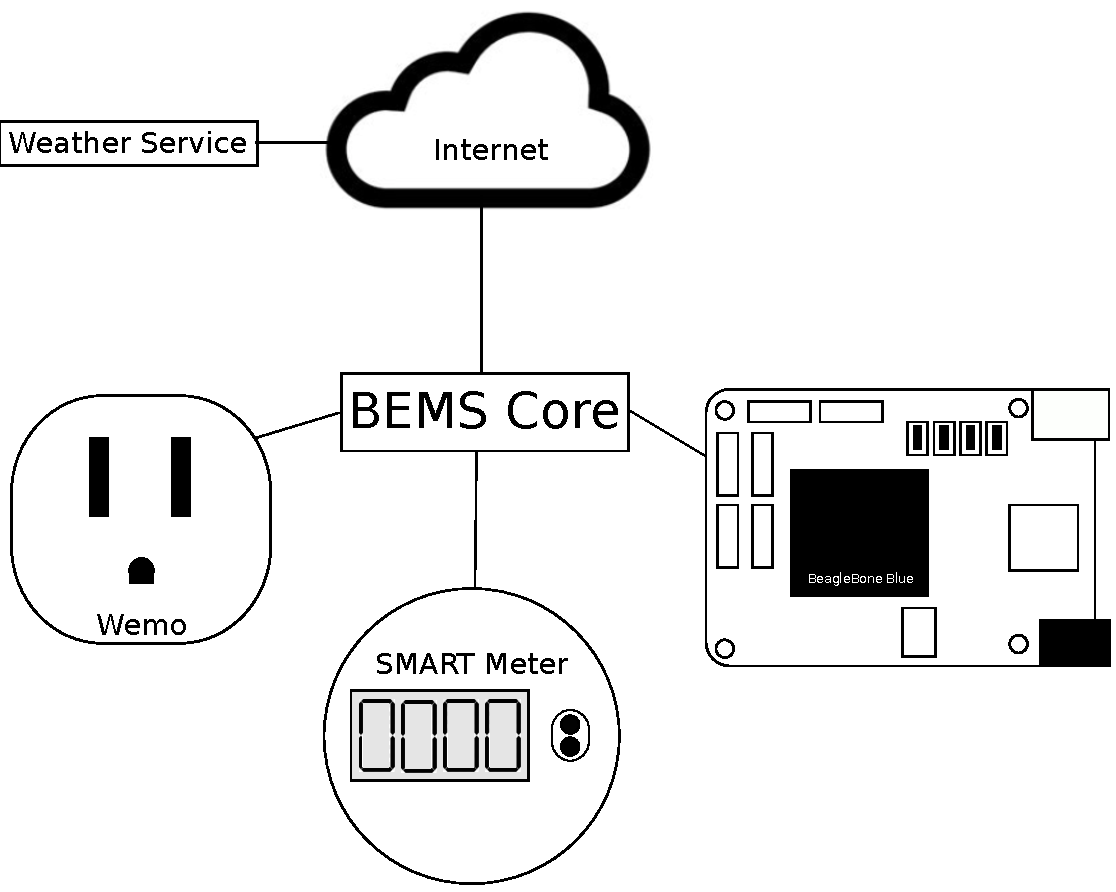
\includegraphics[scale=0.3]{figs/highLevelArchitecture.pdf}
  \caption{High Level Architecture of the Proposed System}
  \label{fig:highLevelArchitecture}
\end{figure}
%
These devices are the WeMo Insight Switch and an embedded computer known as the Beaglebone
Blue. Our initial plan for the smart meter shown in
Figure~\ref{fig:highLevelArchitecture} was to use it in a Simscape model of a
microgrid. However, we did not list this as a requirement for the project, so we
decided not to implement it due to time constraints. The core is also able to
connect the internet to download weather data for Peoria, Illinois through
OpenWeatherMap.

\section{Low Level Architecture}

Figure~\ref{fig:functional_bd} gives lower level detail on the system
architecture. %
%
\begin{figure}
  \centering
  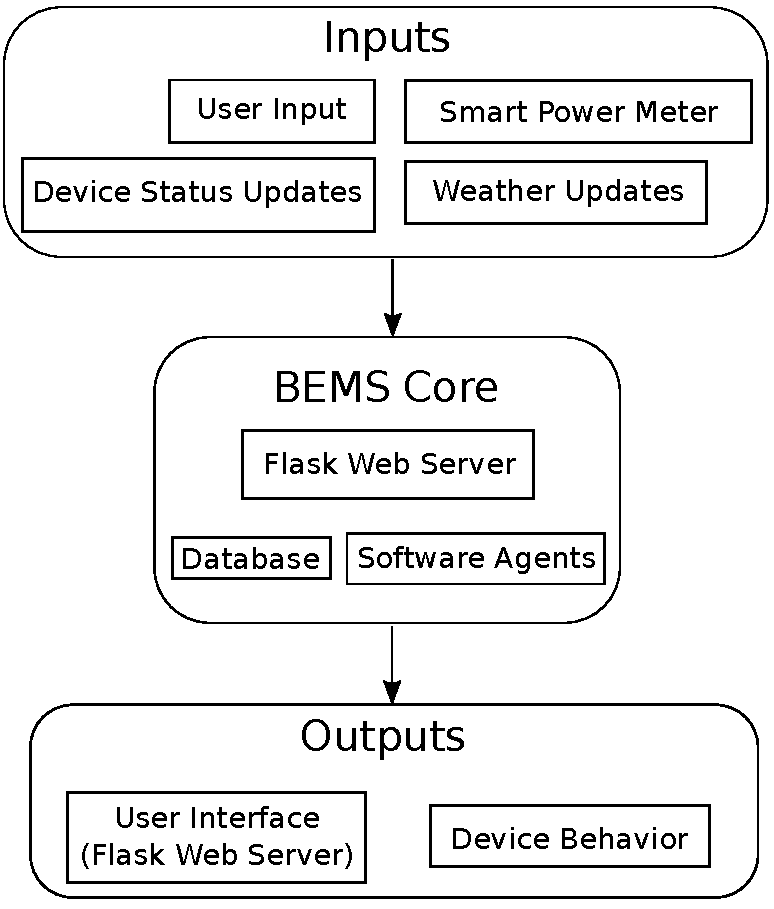
\includegraphics[scale=0.3]{figs/functionalBlockDiagram.pdf}
  \caption{Functional Block Diagram}
  \label{fig:functional_bd}
\end{figure}
%
The inputs include the user input through the web server, the device status
updates (On/Off, power usage, etc...) and the weather data. The iBEMS Core
itself consists of a Flask Web Server, 2 databases (Apache Cassandra and
SQLite), and 3 software agents (Discovery, Control, and Scheduling).


The Flask web server is built using a Python web framework titled Flask which
allows programmers to develop a dynamic web server capable of rendering data to
HTML pages. The benefit of this framework over other Python web frameworks like
Django is the large amount of customization available. For example, the
developers can create a completely custom user login system. For now, the server
is capable of being accessed only on the server computer running Ubuntu Linux.
In the future, support could be added to allow any user on the LAN to access the
web server. Other web frameworks use object relational mapping directly to
access the relevant databases. However, our system uses direct queries with both
SQLite and the Cassandra query language to query the databases. \medbreak We used
2 different databases to store information on. The Apache Cassandra database was
better suited for the time series data such as device status and power usage.
This database was therefore utilized a lot by the Control and Scheduling Agents.
The SQLite database hold parameters that do not change over time like device
ID's, IP addresses, and MAC addresses which made it amendable to the processes
in the Discovery Agent. A possible improvement to this project could be to only
utilize 1 database for development simplicity. \medbreak The first agent that is
used by the iBEMS Core on startup is the discovery agent. It is responsible for
reaching out on the network and finding all devices that the iBEMS Core has
support for. This process involves retrieving the following parameters: IP
address, Port number, MAC address, Manufacturer, Name, and API. Once all
available devices are connected, the Control agent is used to change the status
of each device and collect power usage data in real time. Finally, the
scheduling will take input from the user and place the corresponding scheduling
periods in the Apache Cassandra database. Then, a thread is created to poll the
current device status at regular intervals and update the status if it does not
match the defined status in the Apache Cassandra database.


Figure~\ref{fig:systemComponentInterconnection} provides an explanation of how
the components of the system interact with each other. %
%
\begin{figure}
  \centering
  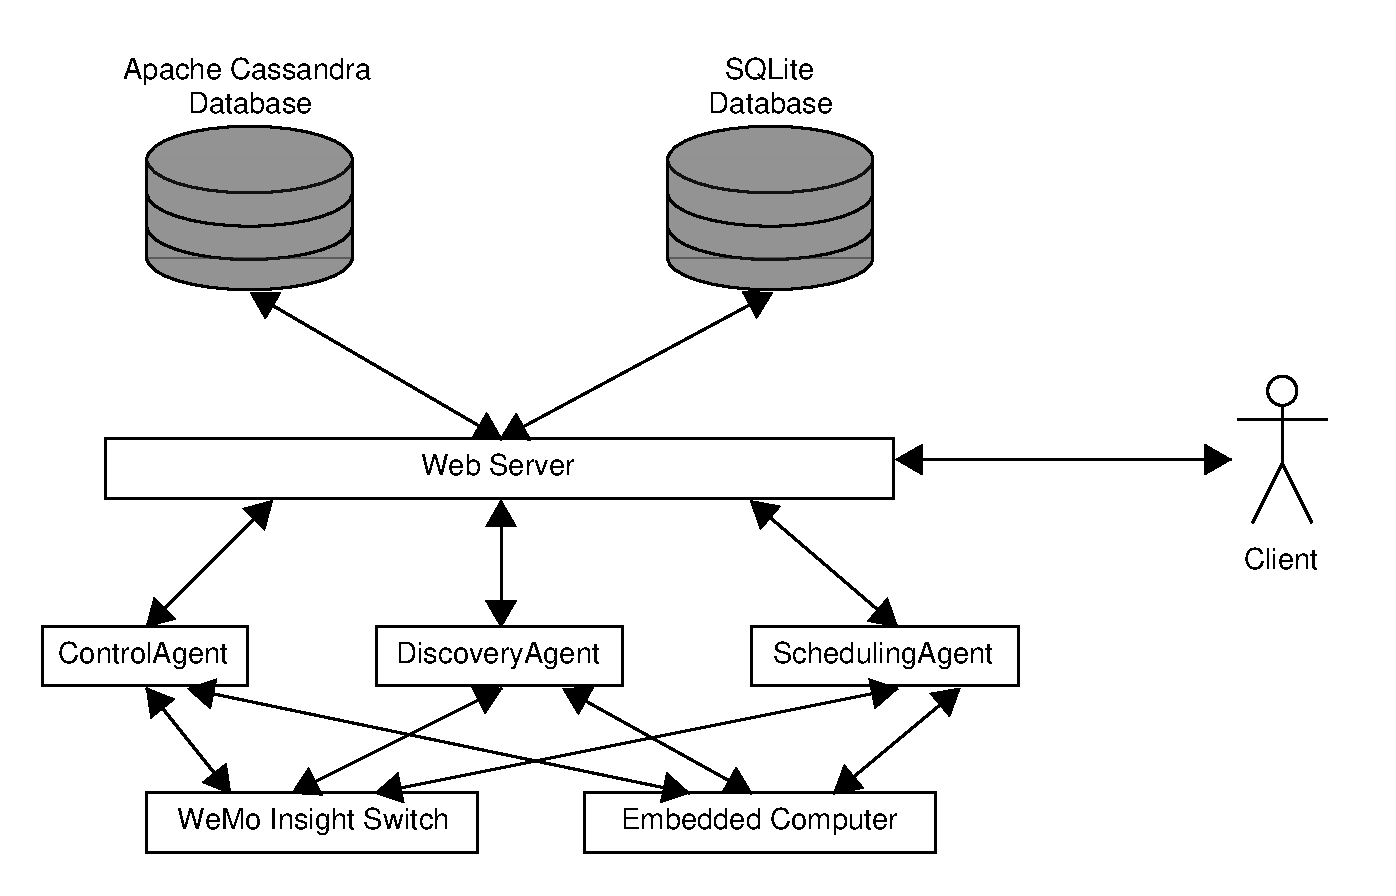
\includegraphics[scale=0.6]{figs/overallDiagram.pdf}
  \caption{Interconnection between system components}
  \label{fig:systemComponentInterconnection}
\end{figure}
%
The Apache Cassandra database and SQLite database are accessible from the web server, control agent, discovery agent, and scheduling agent. The web server queries the time series database and metadata database for vastly different purposes. Power plotting requires querying the Apache Cassandra database. To distinguish between the different devices on the front end, the metadata database is used. The agents utilize the Apache Cassandra database for storing and extracting time-series data. The agents use the metadata database to distinguish between different devices. 

\section{Modes of Operation}


\begin{figure}
  \centering
  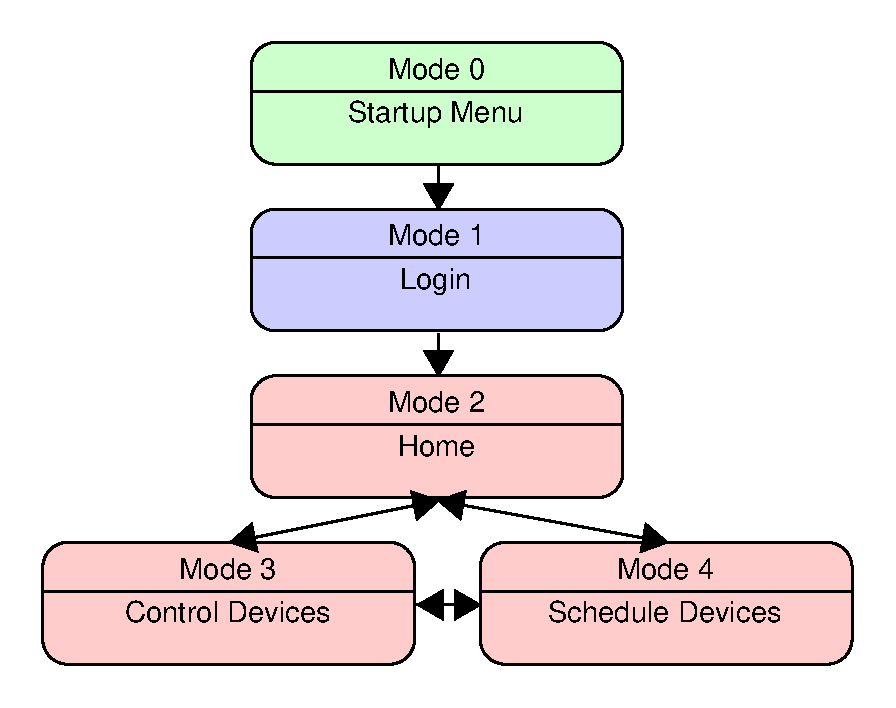
\includegraphics[scale=0.4]{figs/operationalModes.pdf}
  \caption{Operation Modes Interaction}
  \label{fig:operationalModes}
\end{figure}

There are 5 general modes of operation in iBEMS as shown in Figure~\ref{fig:operationalModes}. In Mode 0, before iBEMS is even launched, the user must open the Startup Menu, which is a desktop graphical user interface (GUI). This is a simple GUI with only 2 buttons for starting and stopping iBEMS. Upon clicking \say{Start iBEMS}, the login page will load where the user can enter a valid username and password to use iBEMS. Once a valid username and password is entered, the home screen will be shown which displays the weather data being downloaded from the OpenWeatherMap API. This information includes temperature in Fahrenheit and Celsius, wind speed in MPH, humidity, and cloud coverage. At this point, a navigation bar is available to view the \say{Active Devices} page and the \say{Scheduling} page. \say{Active Devices} corresponds to Mode 3 for controlling devices in real time. The user will also be able to view power plots in this mode as well. Lastly, the \say{Scheduling} page is Mode 4 for creating schedules for all connected devices.

\section{Hardware}

A large feature of this project was being able to record power usage from the
connected IoT devices. The embedded computer does not have a built-in capability
to measure its own power usage, so a circuit was needed to make that
possible. Essentially, this circuit will measure the current being used to drive
one of the motors on the robot chassis. The on-board Analog-to-Digital-Converter
(ADC) can be used to read the voltage across the resistor and since the
resistance is known, the current can be calculated as $I = V/R$. Also, the
voltage from the H-Bridge to drive the motors on the embedded computer is known
so the power consumed by 1 motor is $Motor Drive Voltage * I$. For the specific
robot chassis used in this project, there are 4 motors, so multiplying the power
found from this circuit by 4 will give an approximation of the total power used
by the robot. \add{For other robots with different power sources besides a Lipo
battery.} See Figure~\ref{fig:motorInterfaceCircuit} for details of the interface
circuit for computer power usage by the DC motor. 

\begin{figure}
  \centering
  \begin{circuitikz}[american]
    \tikzstyle{every node} = [font = \tiny]
    % \usetikzlibrary{patterns}
    \draw
    (0,0) to[sqV,invert,l=Motor Drive Voltage from H-Bridge] ++(0,4*\smgrid)
    to[Telmech=M,n=motor,fill=red!20] ++(4*\smgrid,0)
    to[C,l=$1~{[}\mu F{]}$,*-*] ++(0,-4*\smgrid) to[short]++(-4*\smgrid,0); 
    \draw
    (4*\smgrid,4*\smgrid) to[short,-*]++(3*\smgrid,0)
    to[short,-o]++(2*\smgrid,0)node[right]{Embedded Computer ADC (Ch\#0)};
    \draw
    (7*\smgrid,4*\smgrid) to[R,l=$2~{[}\Omega{]}$,-*]++(0,-4*\smgrid)
    to[short]++(-4*\smgrid,0);
    \draw
    (7*\smgrid,0) to[short,-o]++(2*\smgrid,0) node[right]{Embedded
      Computer ADC (Ground)};
  \end{circuitikz}
  \caption{Interface circuit to calculate power consumption of a DC motor
    running from the embedded computer copmuter.}
  \label{fig:motorInterfaceCircuit}
\end{figure}


% \pagebreak
\begin{figure}[H]
    \centering
    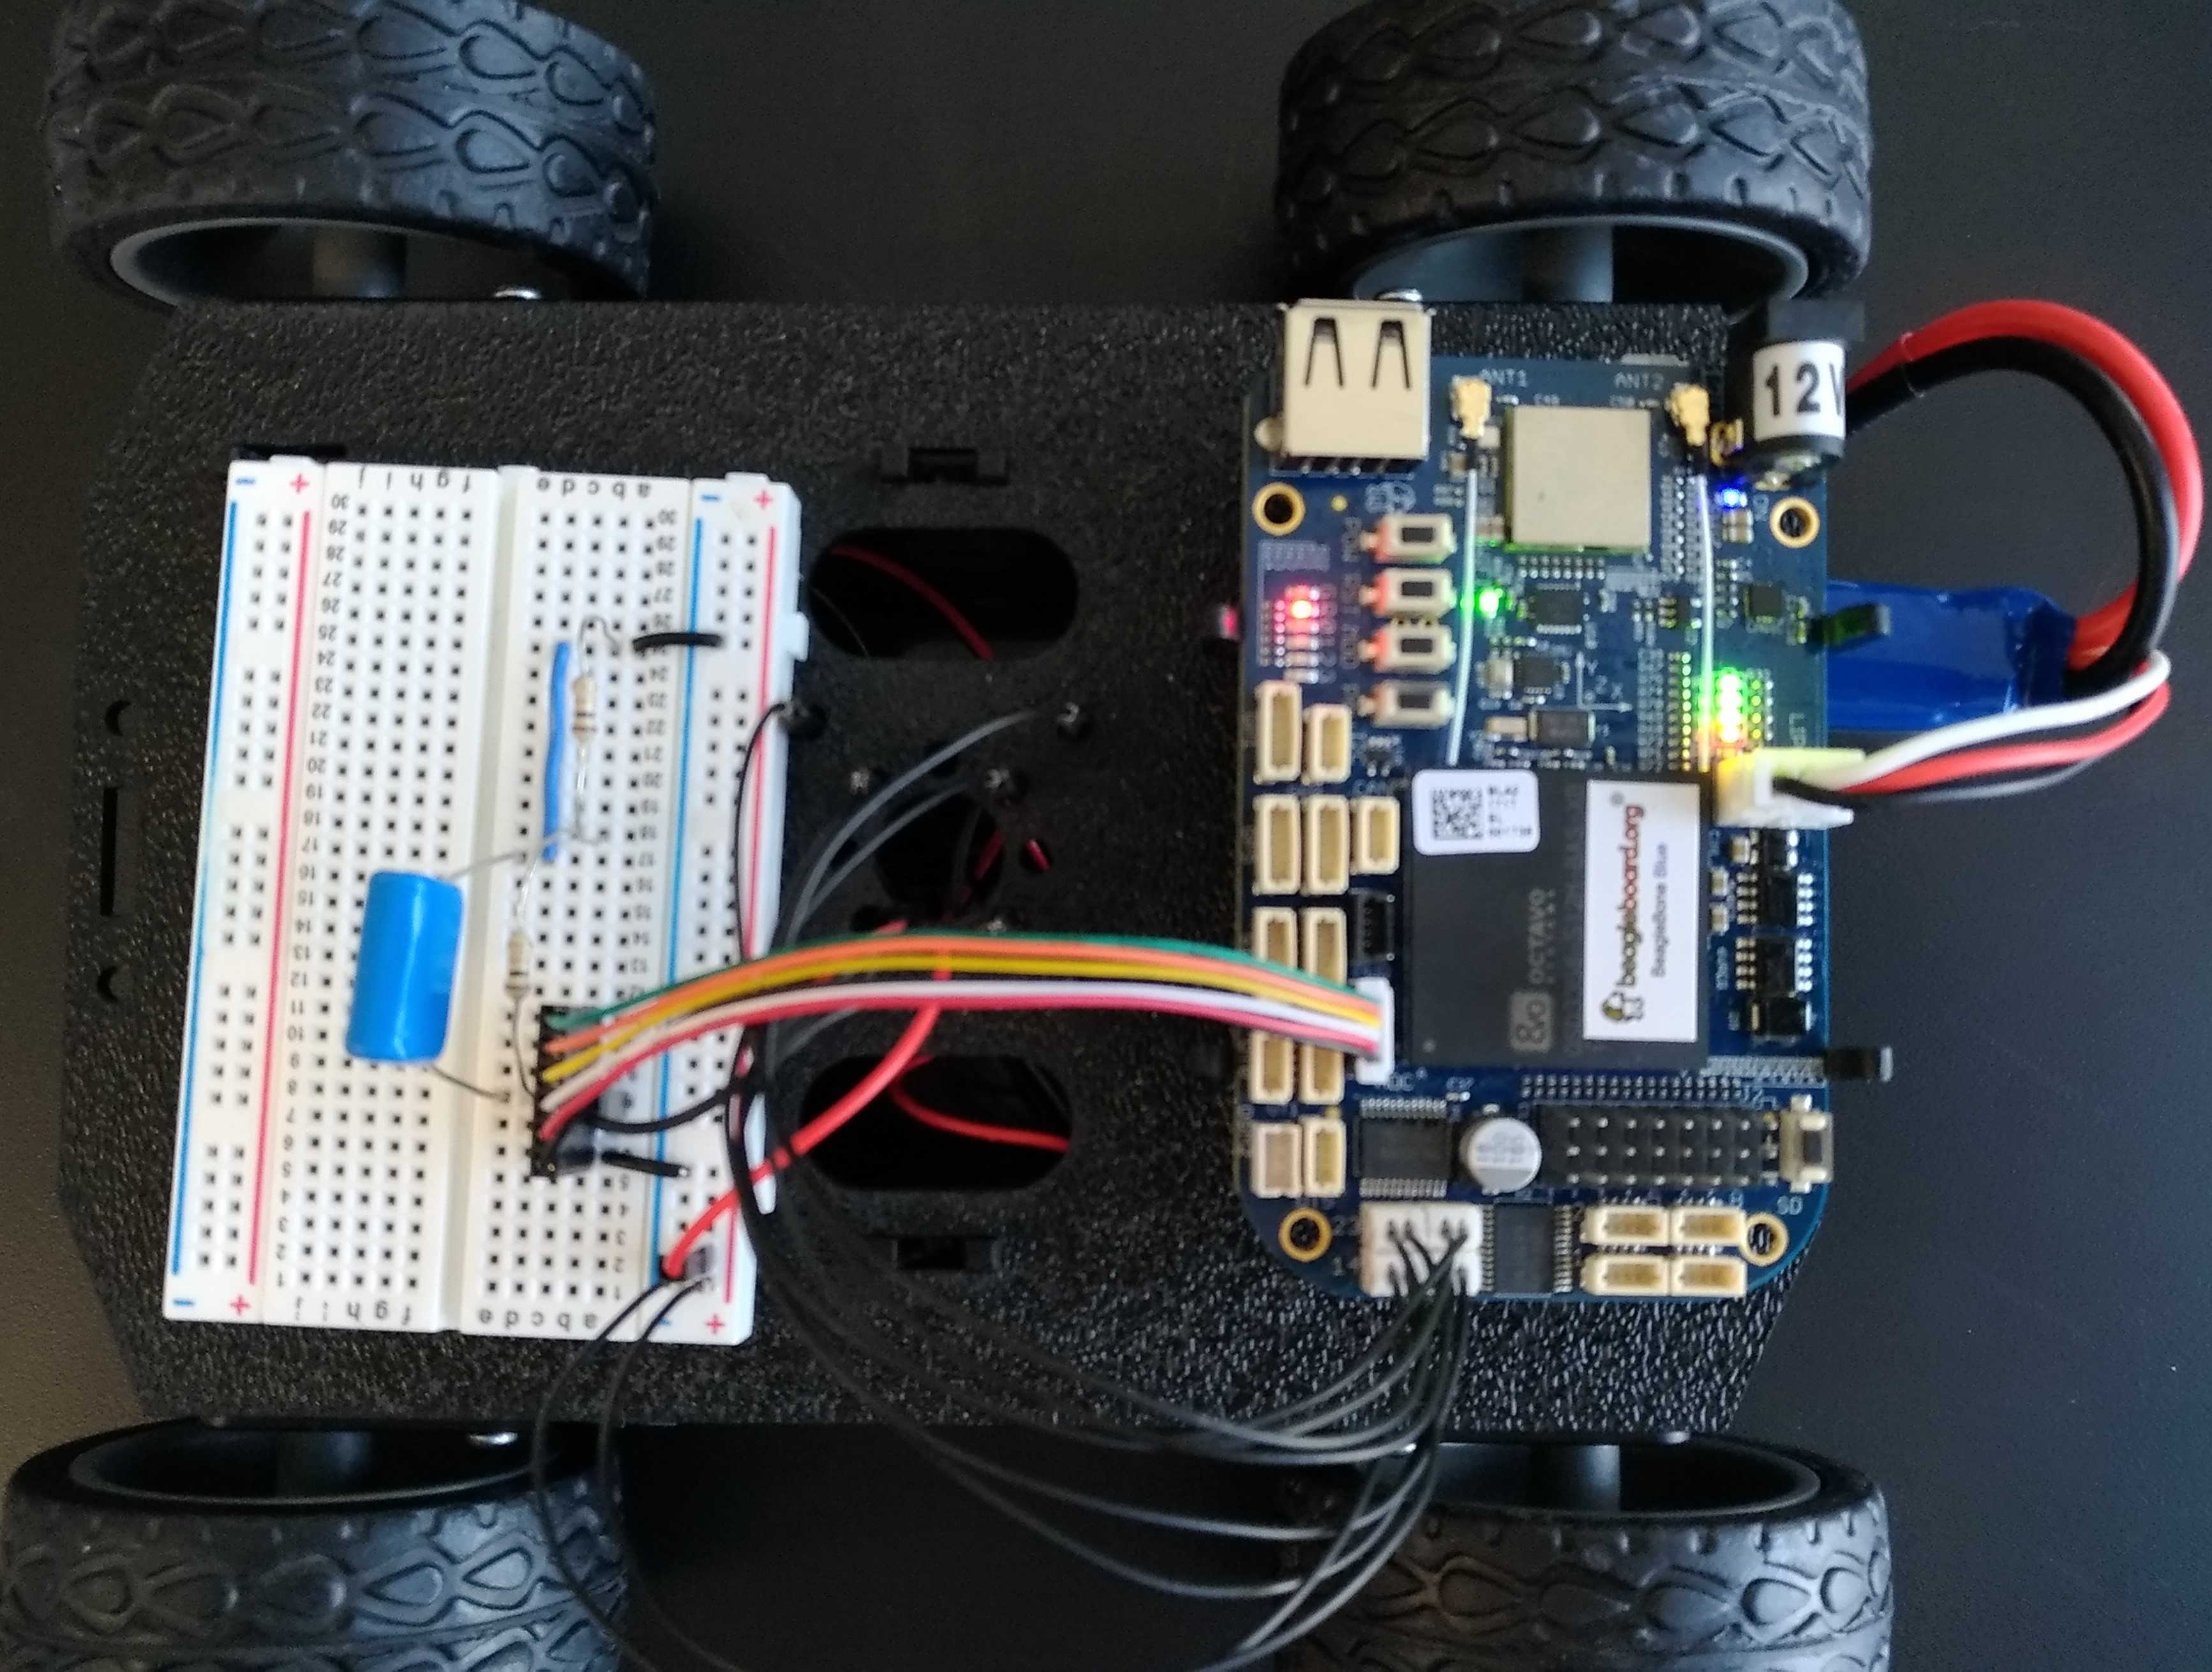
\includegraphics[scale=0.1]{figs/notConnectedSBC.jpg}
    \caption{Embedded Computer Not Connected}
    \label{fig:not_connected_bb}
\end{figure}

Figure~\ref{fig:not_connected_bb} shows the embedded computer mounted on the robot chassis with the circuit shown on page 9. It can also be seen that the embedded computer lights up the on-board red LED when disconnected. Figure~\ref{fig:connected_bb} shows that the embedded computer lights up the green LED when it is connected as an extra indication of its connection status.

\begin{figure}[H]
    \centering
    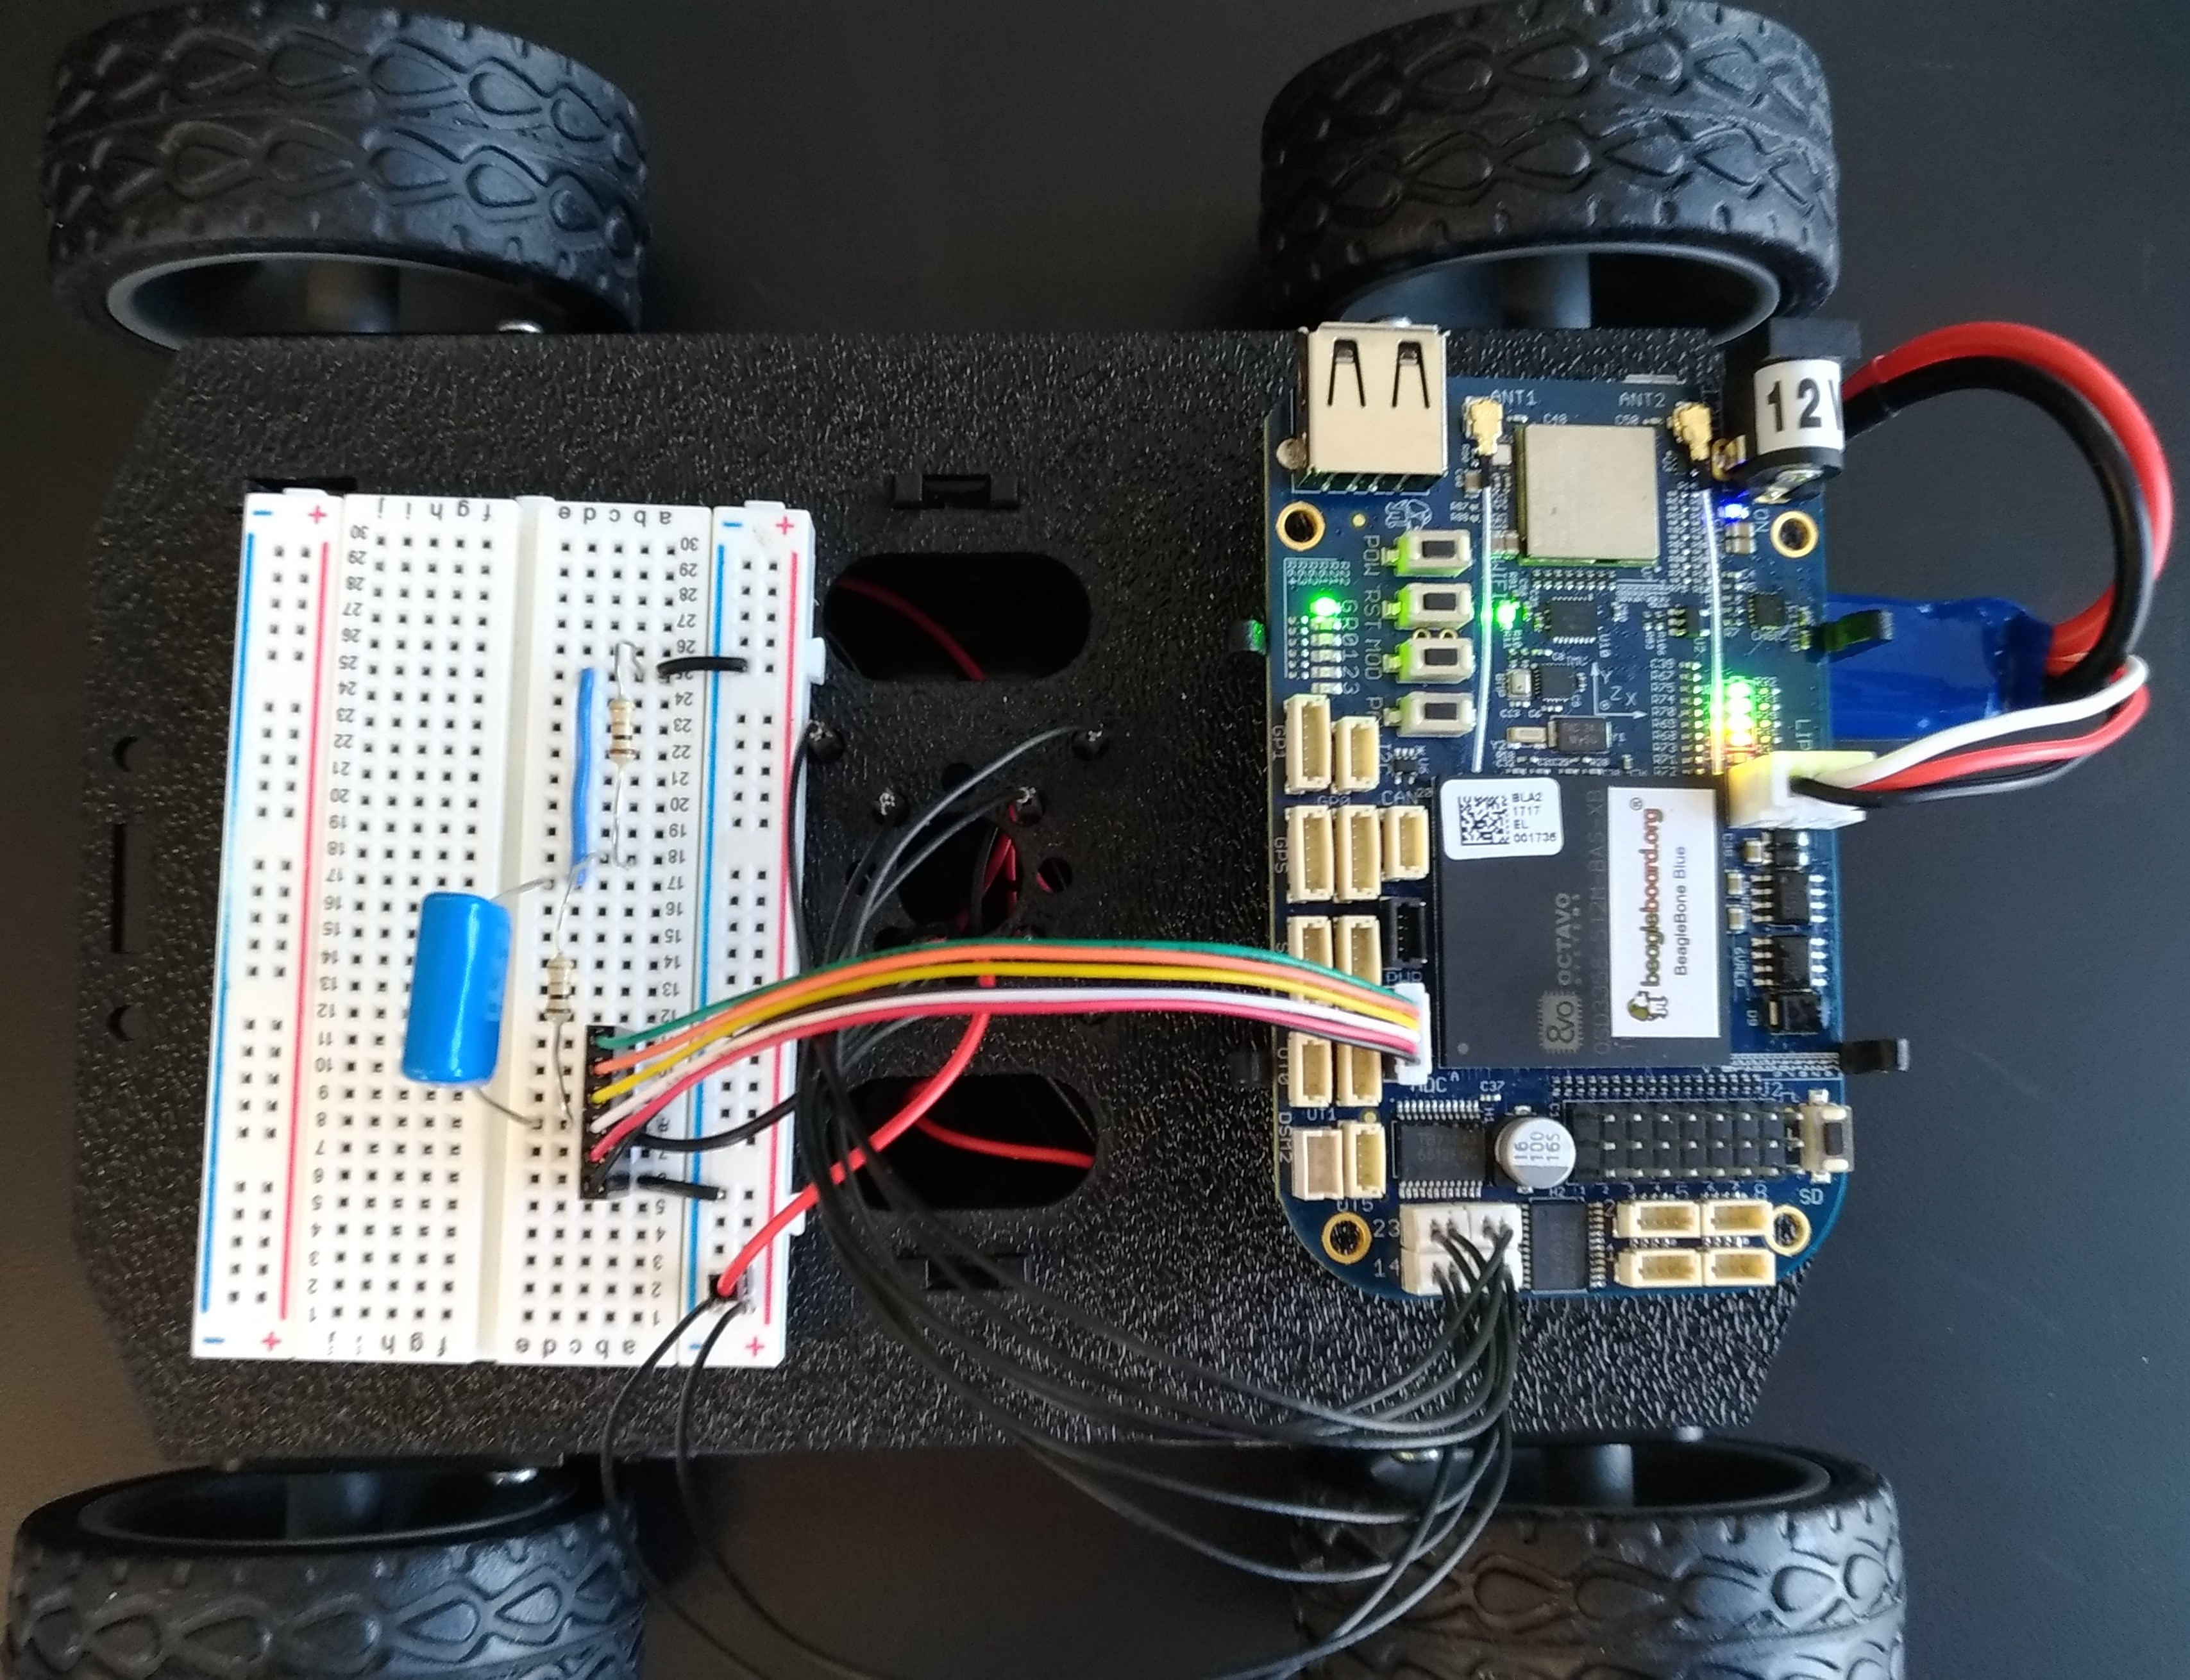
\includegraphics[scale=0.1]{figs/connectedSBC.jpg}
    \caption{Embedded Computer Connected}
    \label{fig:connected_bb}
\end{figure}

\begin{figure}[H]
    \centering
    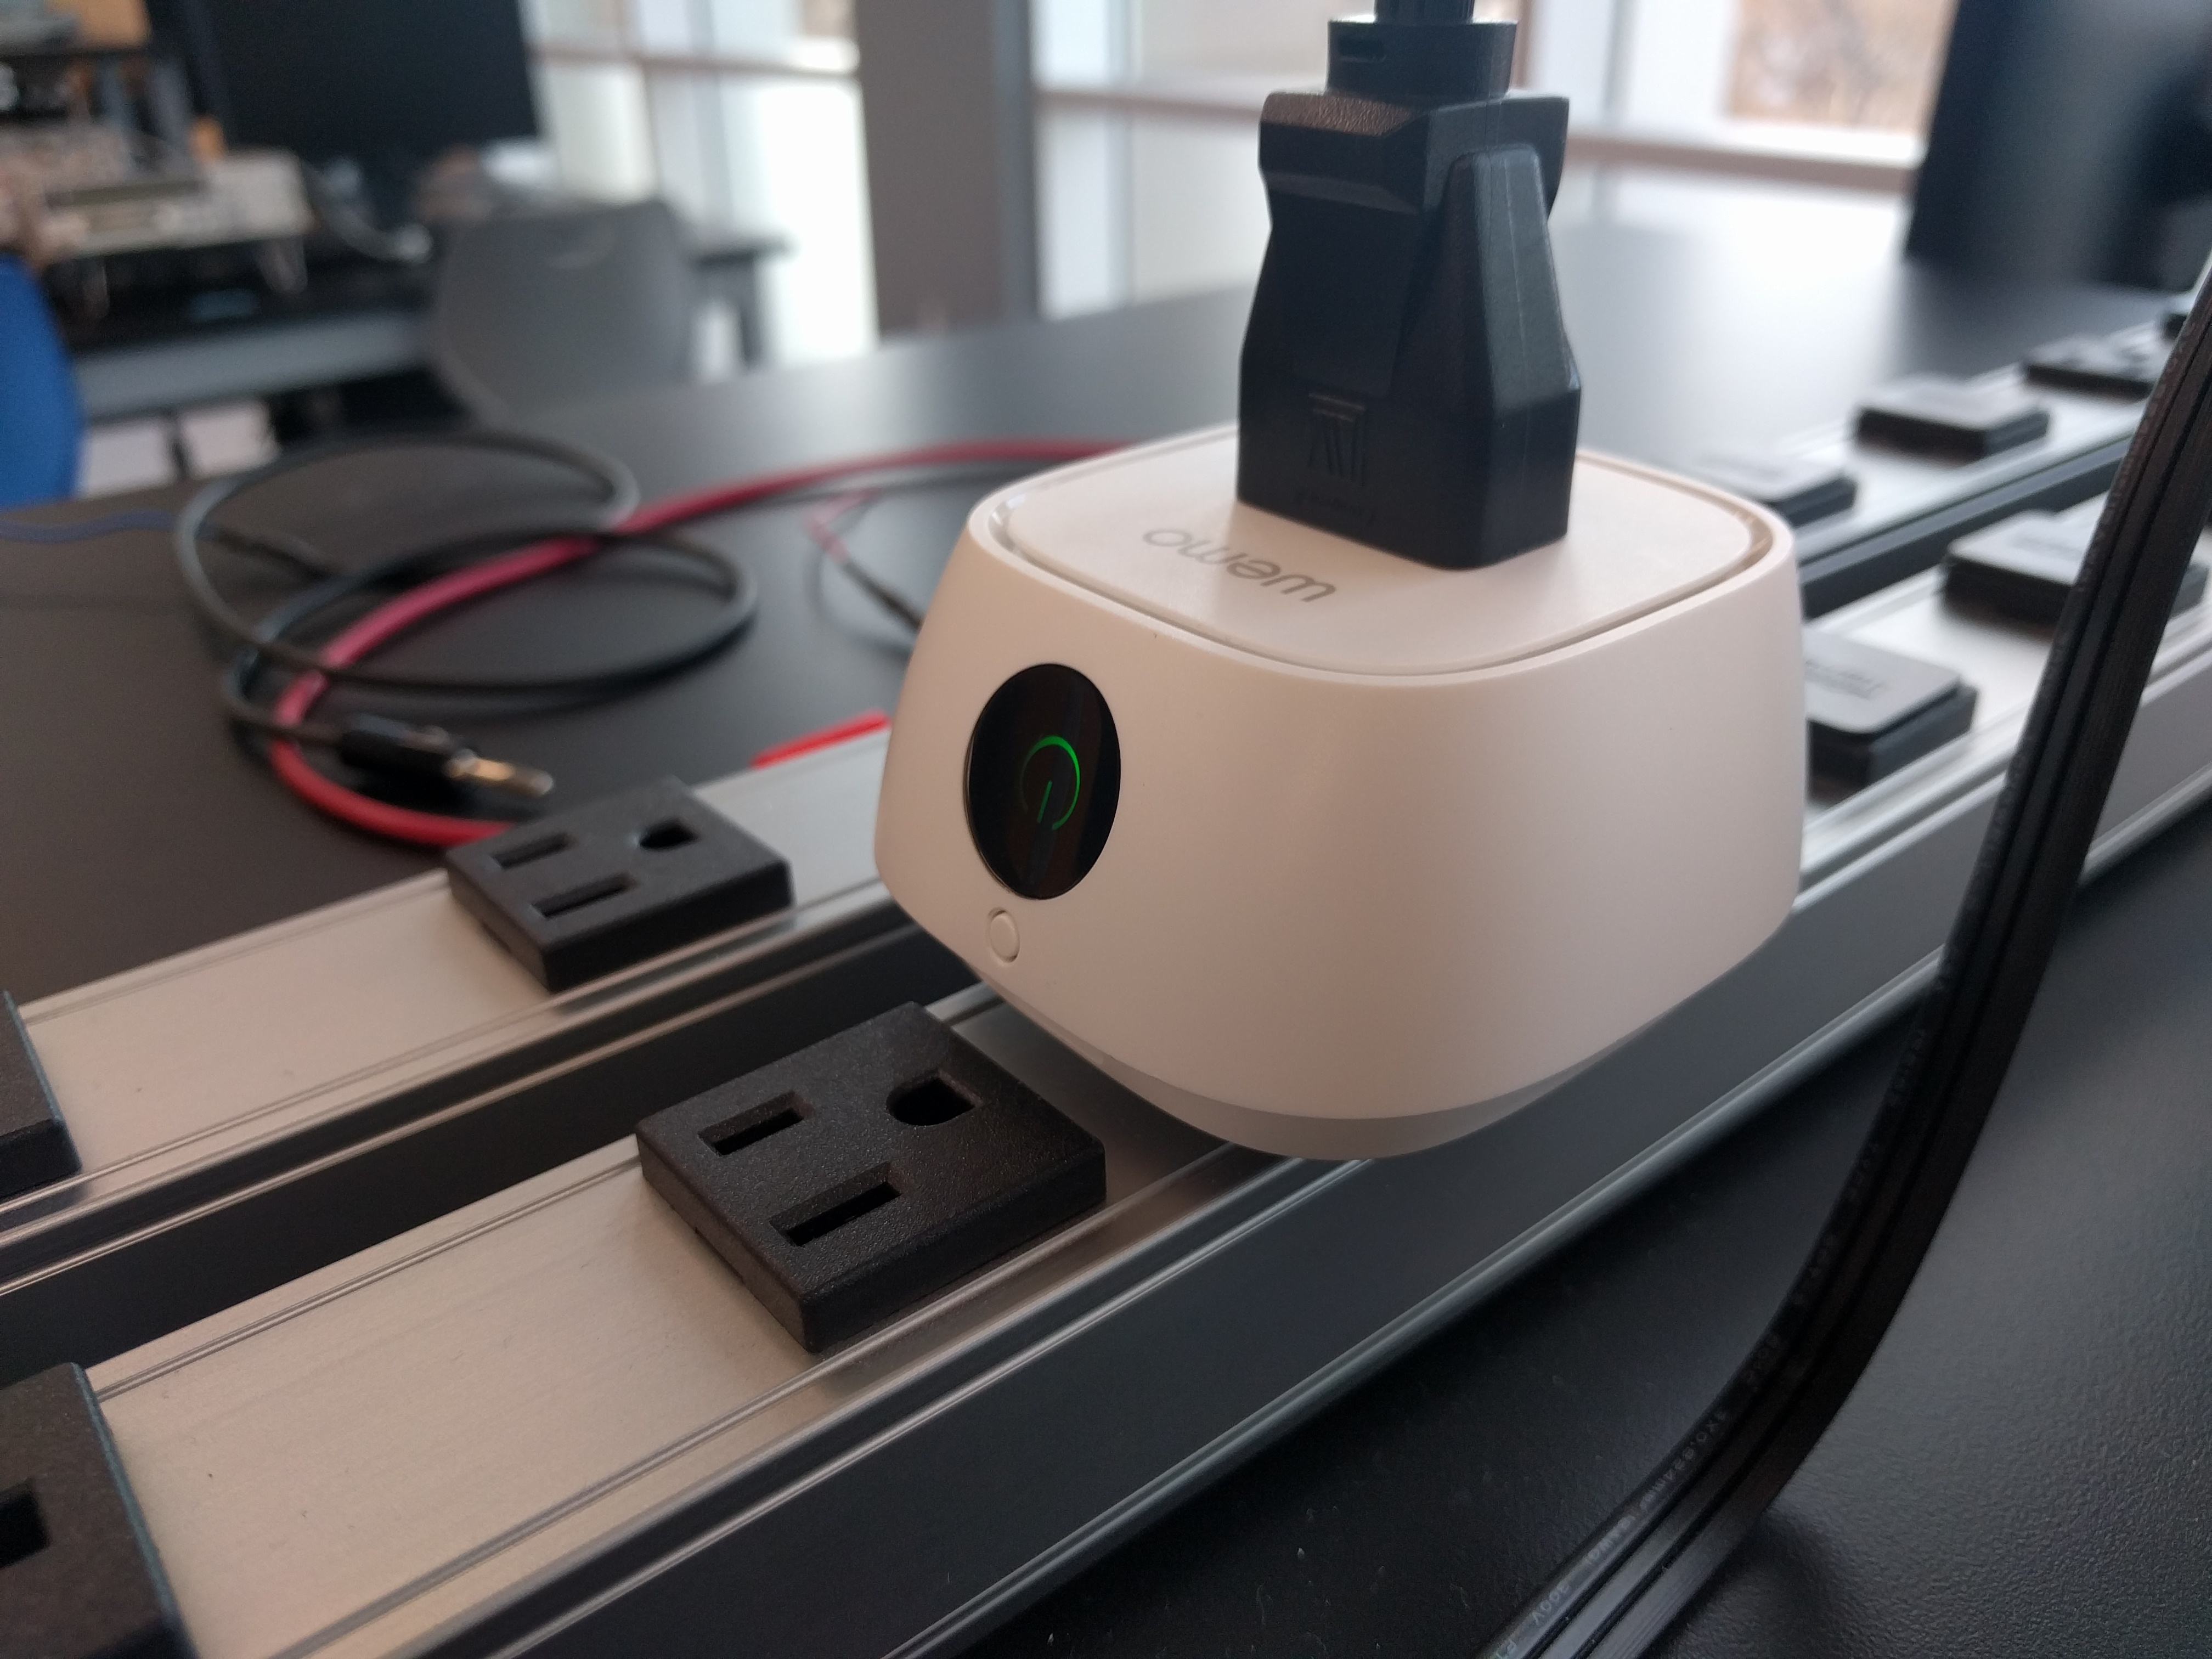
\includegraphics[scale=0.085]{figs/wemoView.jpg}
    \caption{WeMo Insight Smart Plug}
    \label{fig:wemo}
\end{figure}

The other supported device is the WeMo Insight Switch as seen in Figure~\ref{fig:wemo}. This device was easy to develop support for as it is meant for building energy management. It simply plugs into a 120 volt 3-prong outlet and any typical household appliance running on 120 volts can be plugged into it. Internal circuitry allows the WeMo to be controlled remotely (turn On/Off) and to record power usage of whatever it is plugged into.

\begin{figure}[H]
    \centering
    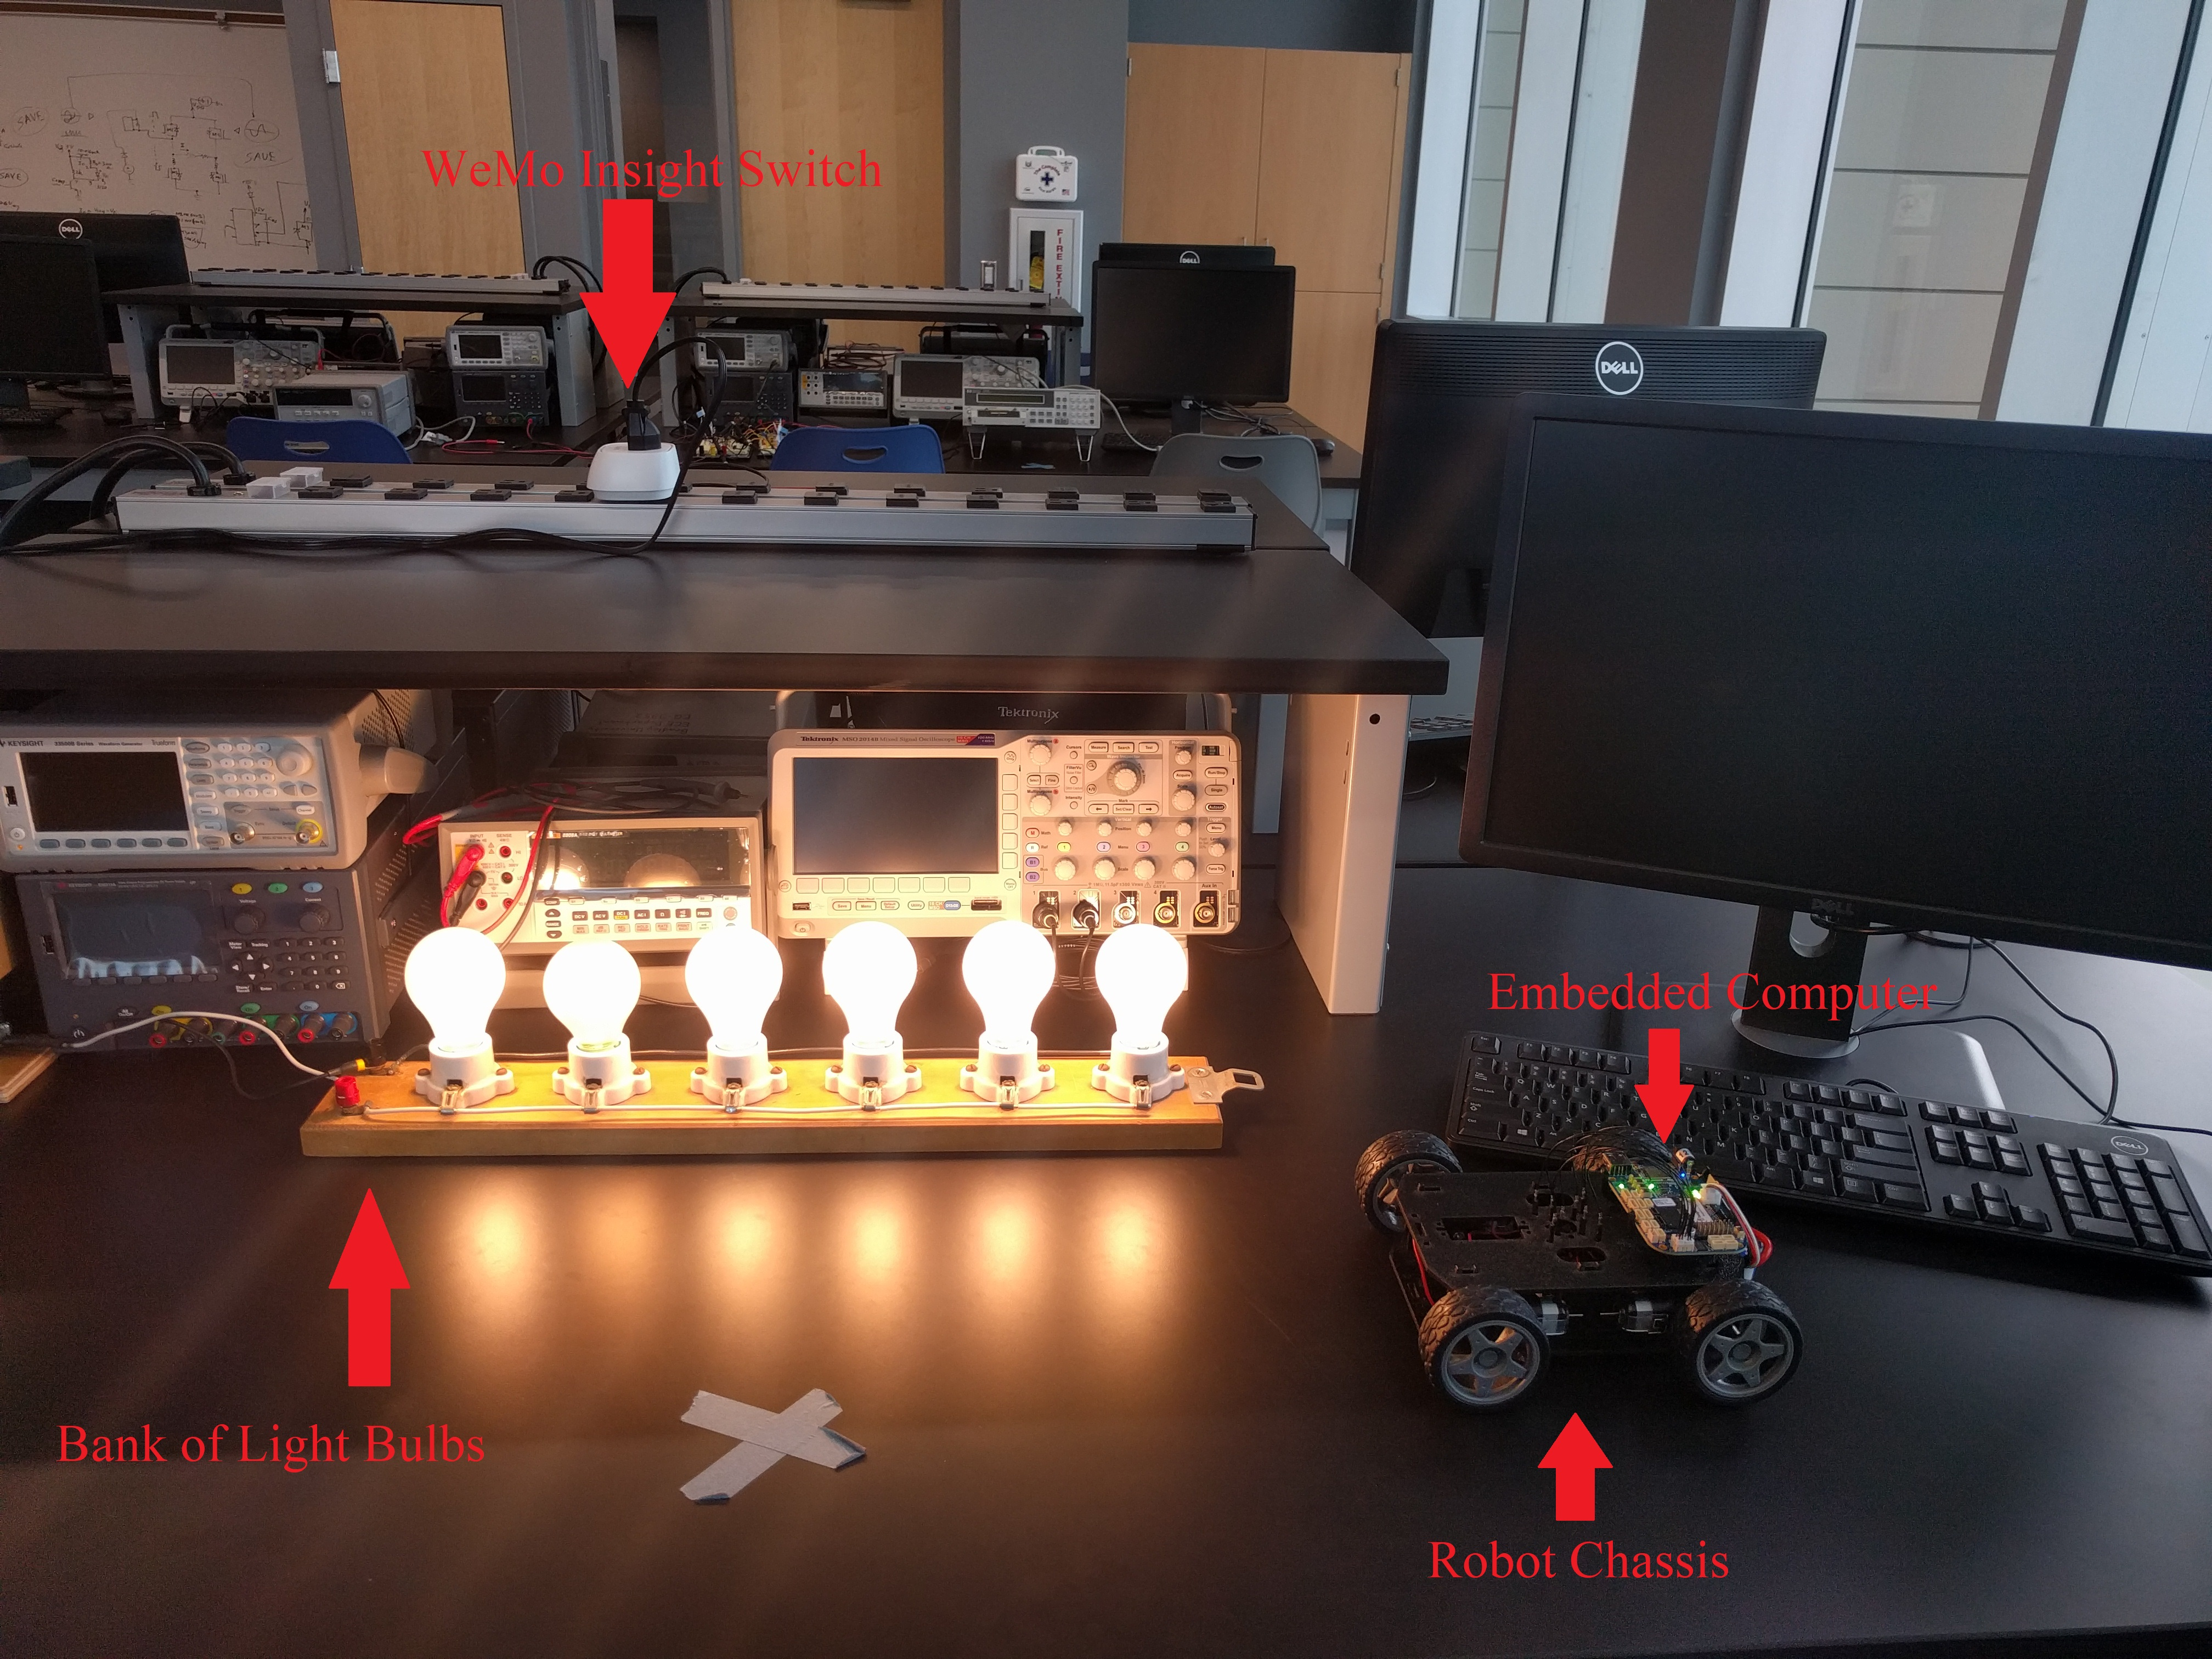
\includegraphics[scale=0.1]{figs/overallView.jpg}
    \caption{Overall View}
    \label{fig:overallView}
\end{figure}

In order to test these devices, we plugged a bank of 6 light bulbs into the WeMo
Insight Switch as seen in Figure~\ref{fig:overallView}. The embedded computer's
functionality was tested with the circuit and robot chassis described earlier.

%%% Local Variables:
%%% mode: latex
%%% TeX-master: "../finalReport"
%%% End:

\chapter{Implementation}
\label{ch: Chapter3}

\section{Agent and Web Server Communication}

% Talk about Zero MQ
All three agents communicate with each other and the web server using the Zero
MQ asynchronous messaging library. Essentially, this library
works as a way to implement inter process communication without a message
broker~\cite{zeromq}. In other words, different processes are able to communicate with each
other without any central bus. This is convenient as fewer processes are needed
for the system to function. Lowering the number of overall processes lowers the
RAM and CPU usage of the software. The library is ported to many different
programming languages; however we are using the Python port titled Pyzmq to
implement in our code base.
%
\begin{figure}
    \centering
    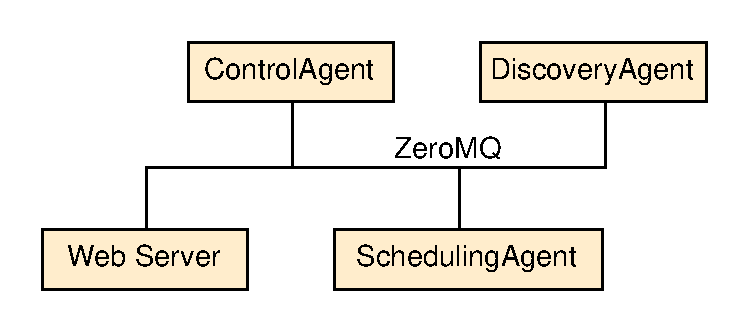
\includegraphics[width=0.4\textwidth]{figs/pubSubAgents.pdf}
    \caption{Publish Subscribe Communication using ZeroMQ}
    \label{fig:pubSubAgents}
\end{figure}

More specifically, the publish subscribe model of communication is used where
each agent communicates via a socket where each socket responds to a specific
topic. The topics and port numbers are listed below along with their
corresponding agents in Table~\ref{tab:pubsubspecs}. %
%
\begin{table}
    \centering
    \begin{tabular}{|c|c|c|}
        \hline
        Agent & Topic & Port Number\\
        \hline
        Discovery Agent & "discovery" & 5556\\
        Scheduling Agent & "scheduling" & 5556\\
        Control Agent & "control" & 5556\\
        \hline
    \end{tabular}
    \caption{Publish/Subscribe Communication Specifications}
    \label{tab:pubsubspecs}
\end{table}
%
In order to send data between the different processes, the topic, method, and
data are delimited in a particular way. This method is shown below as follows: %
%
\begin{verbatim}
    topic method/args
\end{verbatim}
%
A space cannot be included between the method name and arguments as this
interferes with the Python \texttt{split} method for extracting the fields. The
\texttt{topic} is the string described previously, the \texttt{method} is the
name of the desired method to be called on the agent object, and \texttt{args}
is the arguments supplied to the desired method. In order to send a message to
an agent, the \texttt{publish} method defined in the \texttt{pubsub} module
should be called. An optional argument titled \texttt{cycleCount} is available
which will allow the publish message to be sent multiple times. During testing,
it was found that during the transmission of some messages, this was necessary
due to the way ZeroMQ is implemented.

\section{Agent Functionality}
The agents contained in the software are associated with a Python class of the
same name. Each class is instantiated and run with specifications declared in
Table~\ref{tab:pubsubspecs}. Some of the methods defined in each class will be
described in the following subsections.

\subsection{Control Agent Functionality}
The flow chart of method \texttt{setDeviceStatus} is shown in
Figure~\ref{fig:setDeviceStatus}. The purpose of this method is to set the
status of the desired device. When the method is called, the data dictionary is
obtained which contains the device ID. With this device ID, the API type can be
determined using the SQLite database. Subsequently, the appropriate device API
module can be imported. If the power state exists as a key in the device data
dictionary, the power state of the WeMo Insight Switch will be set as ON or OFF.
If the duty cycle key exists, the duty cycle of the single board computer motor
drivers is set. If the shutdown key is set, the single board computer is
shutdown. In order to reconnect to the single board computer, the board must be
started and receiver program ran. If necessary, the device must be reconnected
to the WiFi network. %
%
\begin{figure}
    \centering
    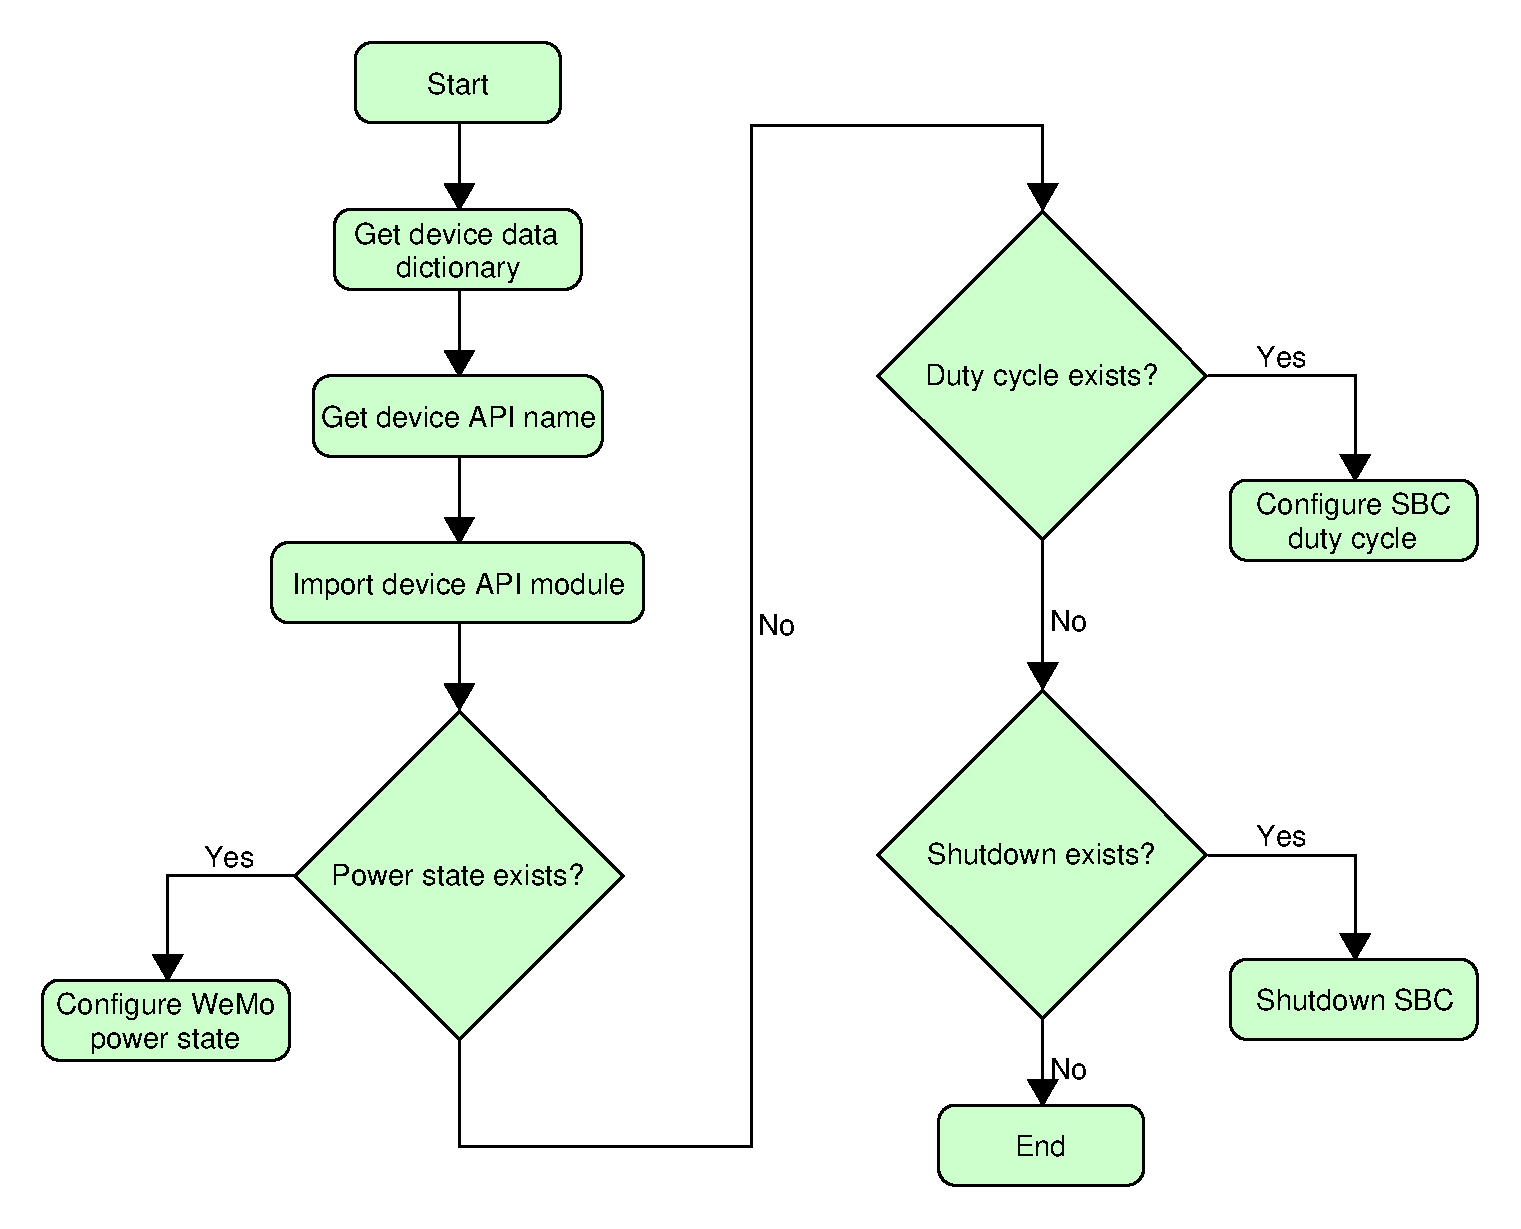
\includegraphics[scale=0.5]{figs/setDeviceStatus.pdf}
    \caption{setDeviceStatus Flow Chart}
    \label{fig:setDeviceStatus}
\end{figure}

To obtain necessary data quantities from the device, the
\texttt{getDeviceStatus} method, defined in Figure~\ref{fig:getDeviceStatus}, is called. Once the proper data parameters are
obtained, the \texttt{getState} function defined in the devices API module can
be called with the data parameters such as power state and
status. Once the agent has finished sending these to the device, a request is
sent to the web server to inform the server that it completed searching for the
required device data. %

%
\begin{figure}
    \centering
    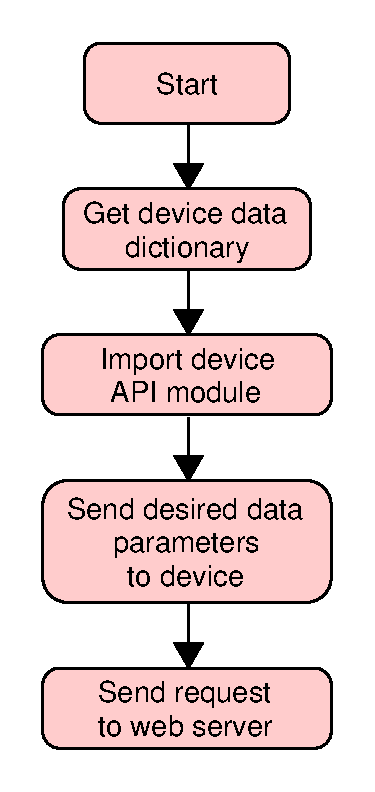
\includegraphics[scale=0.5]{figs/getDeviceStatus.pdf}
    \caption{getDeviceStatus Flow Chart}
    \label{fig:getDeviceStatus}
\end{figure}

Every device connected to iBEMS will have a thread associated with it started from the control agent. This thread will run the \texttt{periodicQueryBehavior} method to periodically query for device data and store in the corresponding Cassandra database table. A user specified delay is placed in the class's module to prevent the thread from overwhelming the system.
\begin{figure}[H]
    \centering
    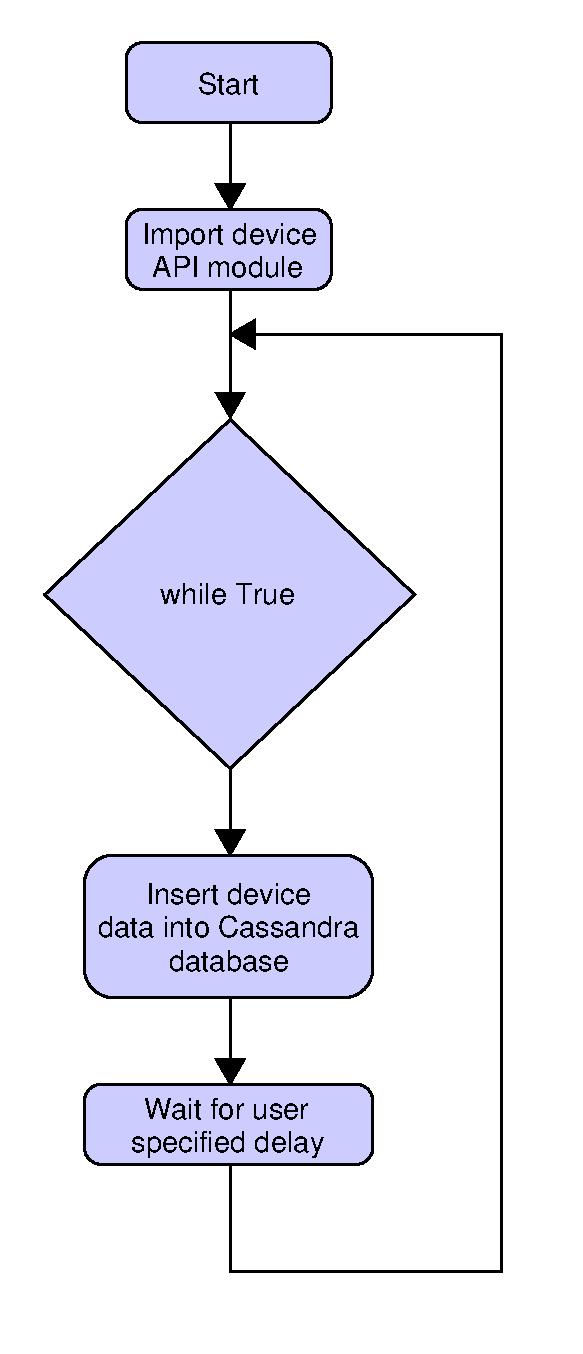
\includegraphics[scale=0.5]{figs/periodicQueryBehavior.pdf}
    \caption{periodicQueryBehavior Flow Chart}
    \label{fig:periodicQueryBehavior}
\end{figure}
To reduce latency, the device status is retrieved directly from the API module in the \texttt{periodicQueryBehavior} method rather than calling \texttt{getDeviceStatus} as this prevents the API from being imported unnecessarily.

\subsection{Discovery Agent Functionality}
The purpose of the discovery agent is to search for devices that respond to the supported APIs by the software. A flow chart demonstrating the \texttt{searchForDevices} method is shown in Figure~\ref{fig:searchForDevices}. This method is called whenever the active devices page is loaded. The algorithm could be improved to help page load times. All the device APIs are loaded by the \texttt{findDevices} function which will return a list of found URLs. Once the device's URL is determined, it's metadata can be passed to the \texttt{setDeviceToActive} method which will set up the device in the two databases.

\begin{figure}[H]
    \centering
    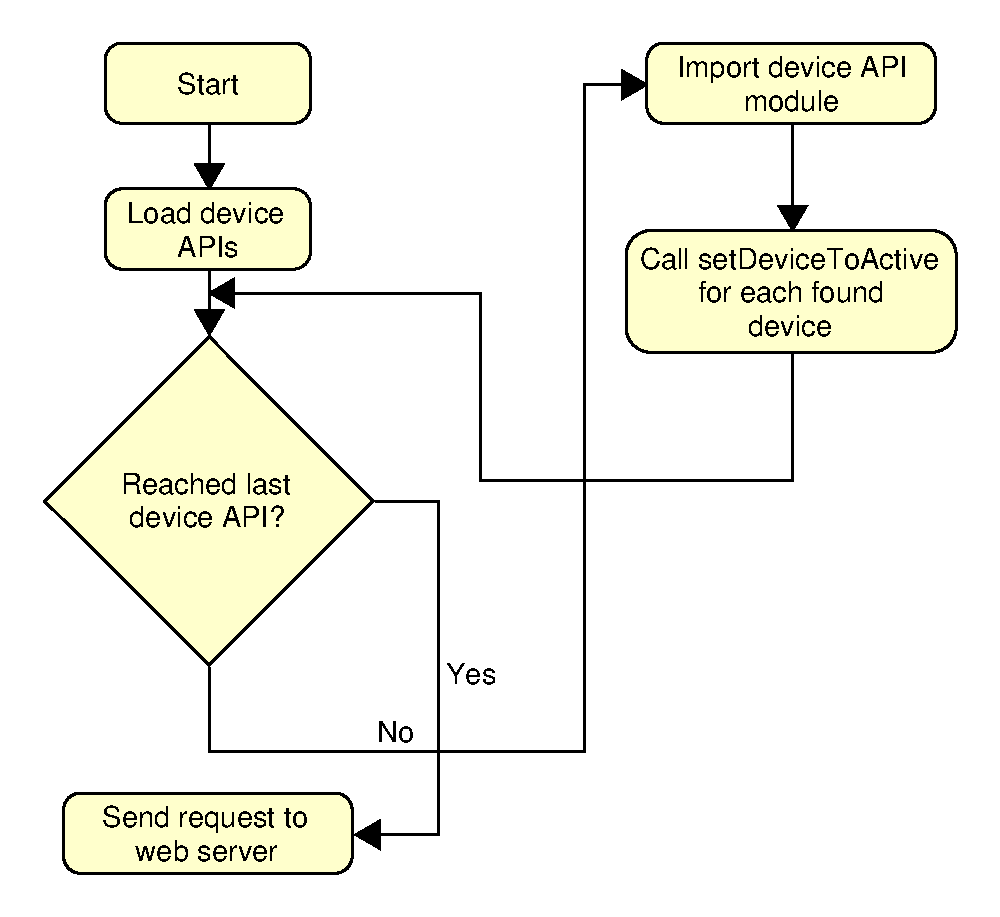
\includegraphics[scale=0.5]{figs/searchForDevices.pdf}
    \caption{searchForDevices Flow Chart}
    \label{fig:searchForDevices}
\end{figure}
The \texttt{setDeviceToActive} method shown in Figure~\ref{fig:setDeviceToActive} will first check to make sure the device is not already in the active devices table. Then, it will add the device to the active devices table, create a table in the Cassandra database for storing time-series data, send a message to the scheduling agent to check for schedule updates, and send a message to the control agent to start collecting data.
\begin{figure}[H]
    \centering
    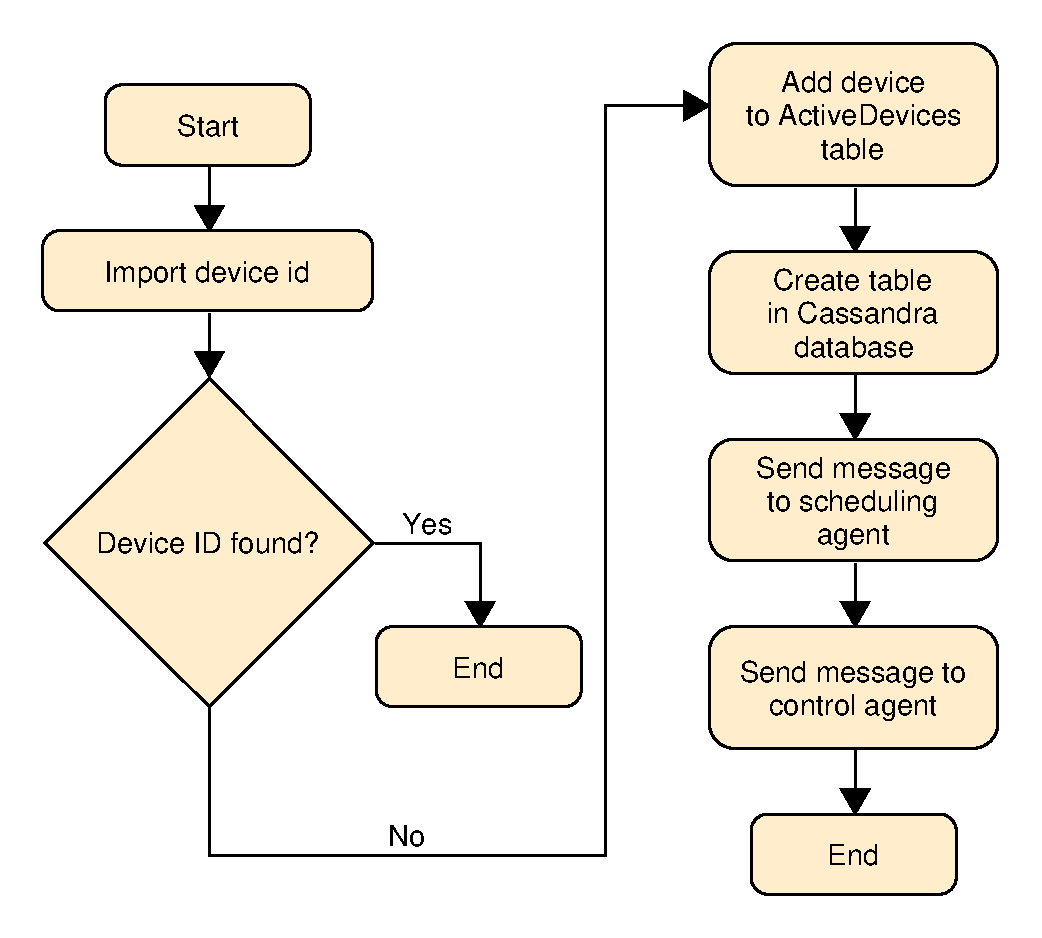
\includegraphics[scale=0.5]{figs/setDeviceToActive.pdf}
    \caption{setDeviceToActive Flow Chart}
    \label{fig:setDeviceToActive}
\end{figure}

\subsection{Scheduling Agent Functionality}
The scheduling agent is able to update the device status of each device dependent on whether a schedule is set for the specific time period and day. One of the methods that is called, \texttt{updateScheduleFromServer} is invoked when the user presses the \say{Update Schedule} button from the UI on the scheduling page. A flow chart of this method is shown in Figure~\ref{fig:updateScheduleFromServer}. When this method is called the desired schedule is loaded in as a dictionary and parsed to extract the necessary periods and given day. First the times are stored in military time in the database for more convenient storage and parsing later on. Then, a table is created in the Apache Cassandra database where the device ID and day are embedded in the name. The previous table's data is destroyed to ensure there are no errors regarding overlapping schedules. Lastly, all the scheduling periods extracted from the dictionary are stored as rows in the table. 
\begin{figure}[H]
    \centering
    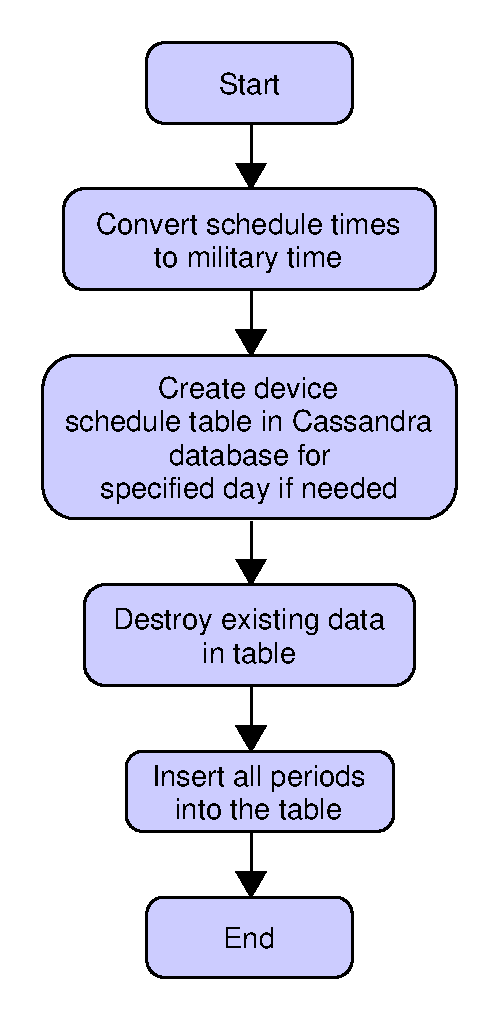
\includegraphics[scale=0.5]{figs/updateScheduleFromServer.pdf}
    \caption{updateScheduleFromServer Flow Chart}
    \label{fig:updateScheduleFromServer}
\end{figure}
A second method that is run inside each device thread is \texttt{periodicDeviceUpdateMethod}, defined in Figure~\ref{fig:periodicDeviceUpdateMethod}, which is started when the discovery agent sets the discovered device to active. By first loading the device's API name, the scheduling agent can begin checking for scheduling periods inside an infinite loop. The status dictionary is queried from the Cassandra database and loaded into a dictionary. All these scheduling periods are looped over for the current day while constantly checking whether the current time in seconds is within the starting and ending time. A conversion of both starting and ending time to seconds is necessary as it is challenging to work with these quantities in standard and military time when comparing times. If the current time does lie inside the scheduling period, the device's state is set dependent on the API. 
\begin{figure}[H]
    \centering
    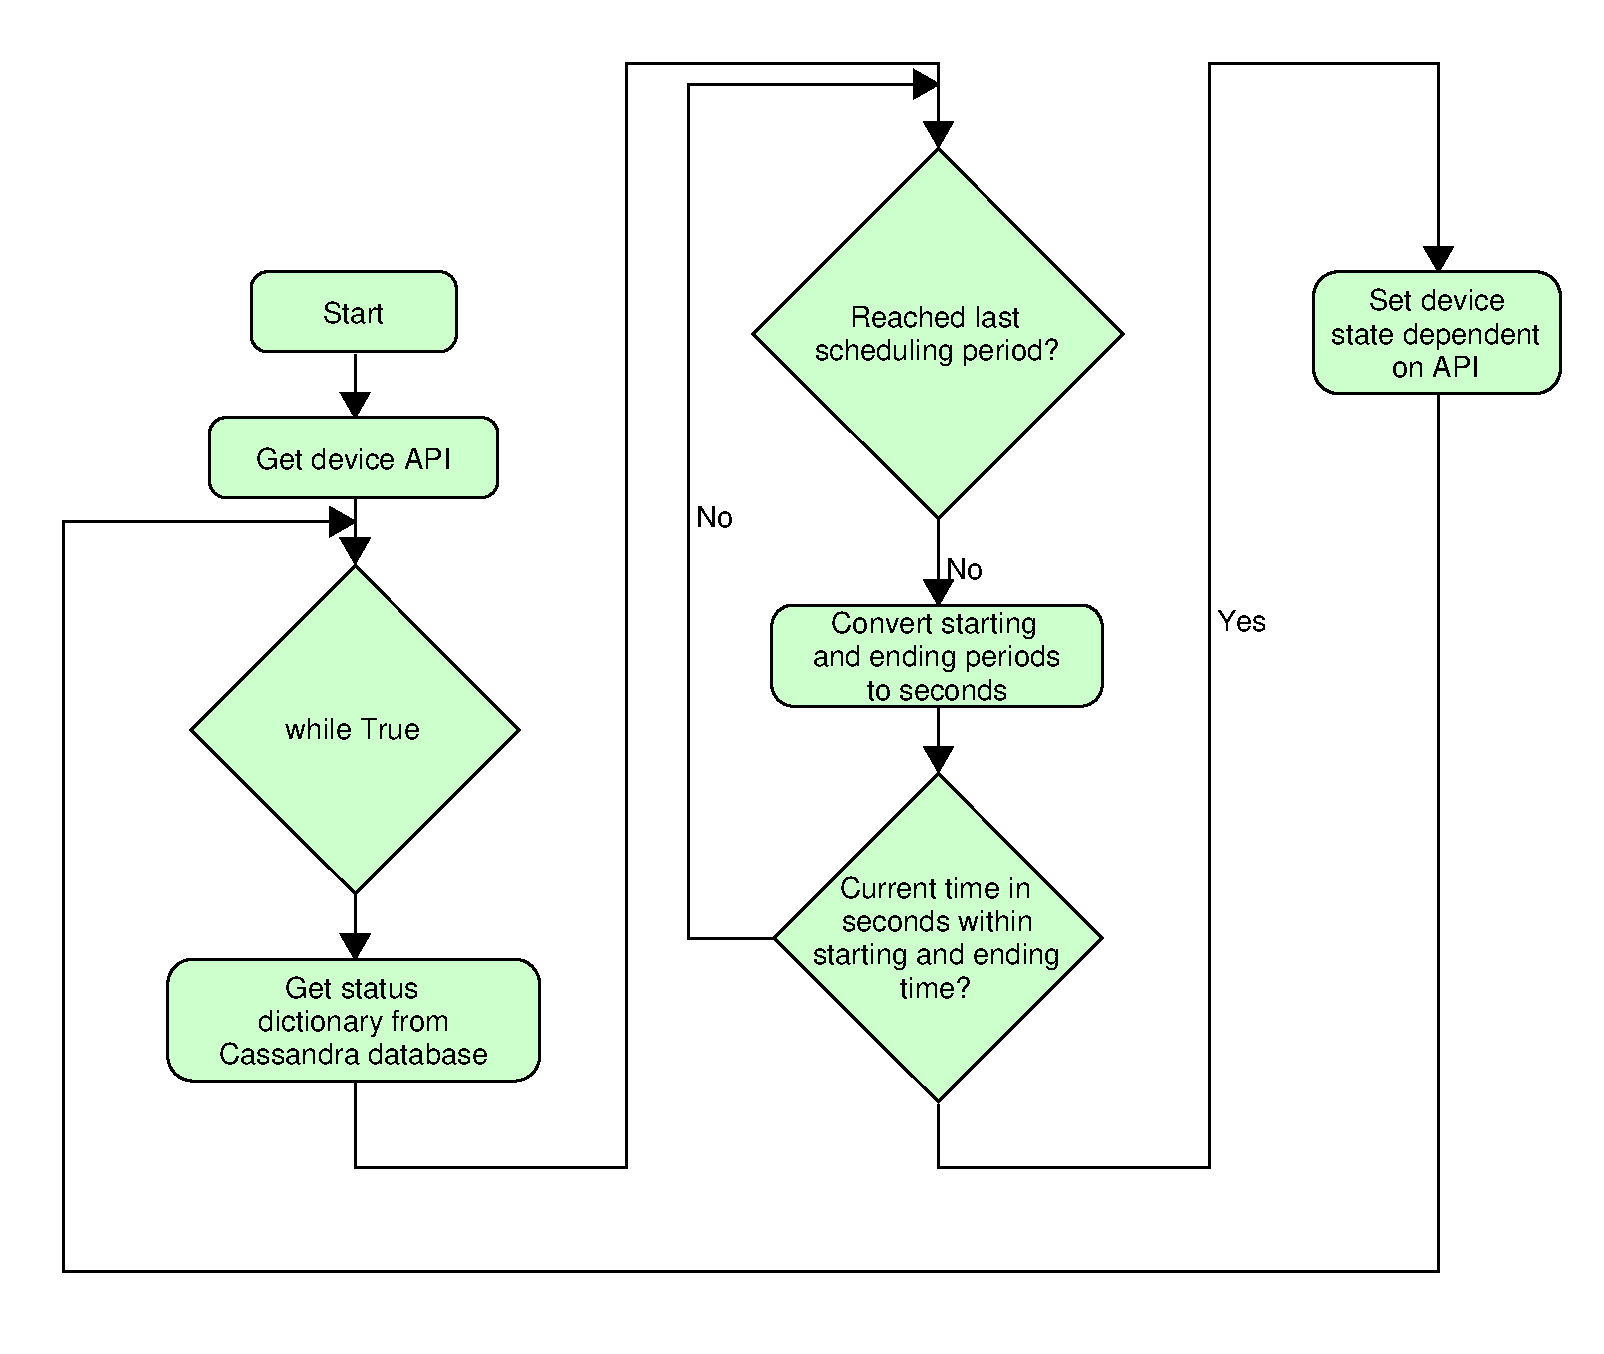
\includegraphics[scale=0.5]{figs/periodicDeviceUpdateMethod.pdf}
    \caption{periodicDeviceUpdateMethod Flow Chart}
    \label{fig:periodicDeviceUpdateMethod}
\end{figure}

\section{Desktop GUI Functionality}
The functionality of the desktop GUI launched when the user runs the Python script titled \texttt{GUI.py} is shown in Figure~\ref{fig:desktopgui}. Packages used to construct the GUI include tkinter which is a Python interface for the Tcl/Tk GUI toolkit. When the GUI is started up, the title, buttons, and labels are created along with ties to the callback functions \texttt{startCallback} and \texttt{stopCallback}. The \texttt{startCallback} function is called when the user presses the \say{Start iBEMS} button. This function first checks whether iBEMS is already running by checking for processes already running on the machine including the web server itself and the three agents. This is performed using the command \texttt{ps -aux}. After this has been completed, an error popup is shown preventing another instance of the software from running. This prevents errors associated with copies of agents and web servers running simultaneously. To properly stop the software, the \say{Stop iBEMS} button will shutdown the software by first finding the process ID's associated with the agents and web server. To perform this, it will place the output of \texttt{ps -aux | grep [process]} into a text file where \say{process} is the name of the target process. A file descriptor of the process status output text file is instantiated and all the lines are read in to be parsed. Each process output is split by spaces and the second element in the list is denoted as the process id. Then, using the \texttt{kill} command, these processes are killed. 
\begin{figure}[H]
    \centering
    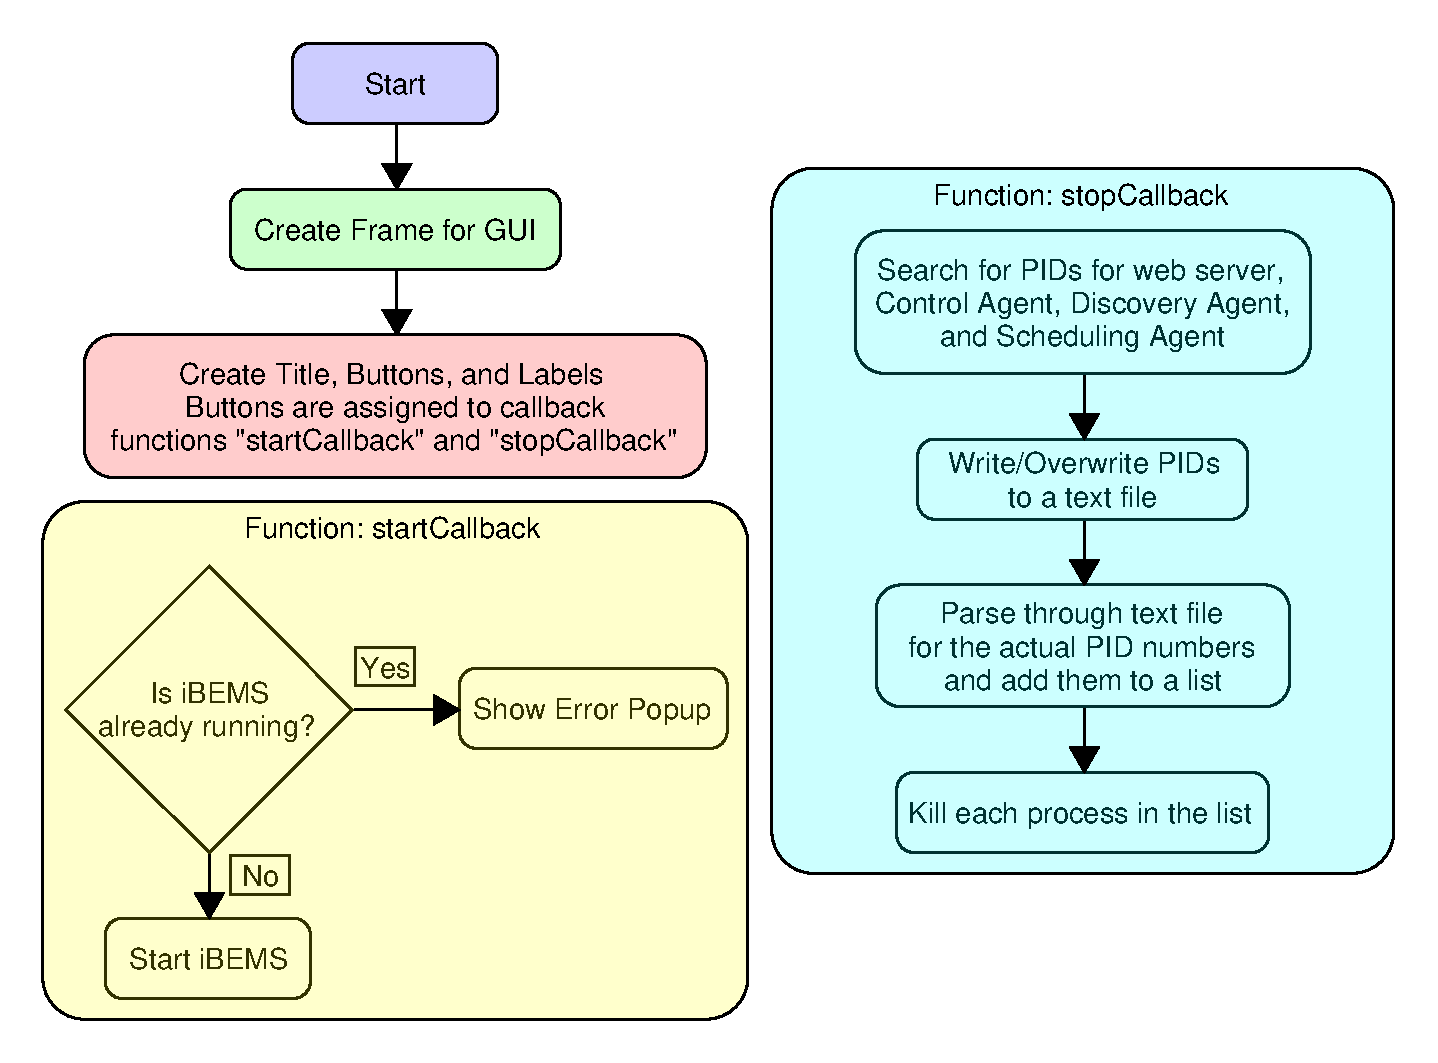
\includegraphics[scale=0.6]{figs/GUI_Diagram.pdf}
    \caption{Python desktop GUI Functionality}
    \label{fig:desktopgui}
\end{figure}

\section{Embedded Computer}

\begin{figure}[H]
    \centering
    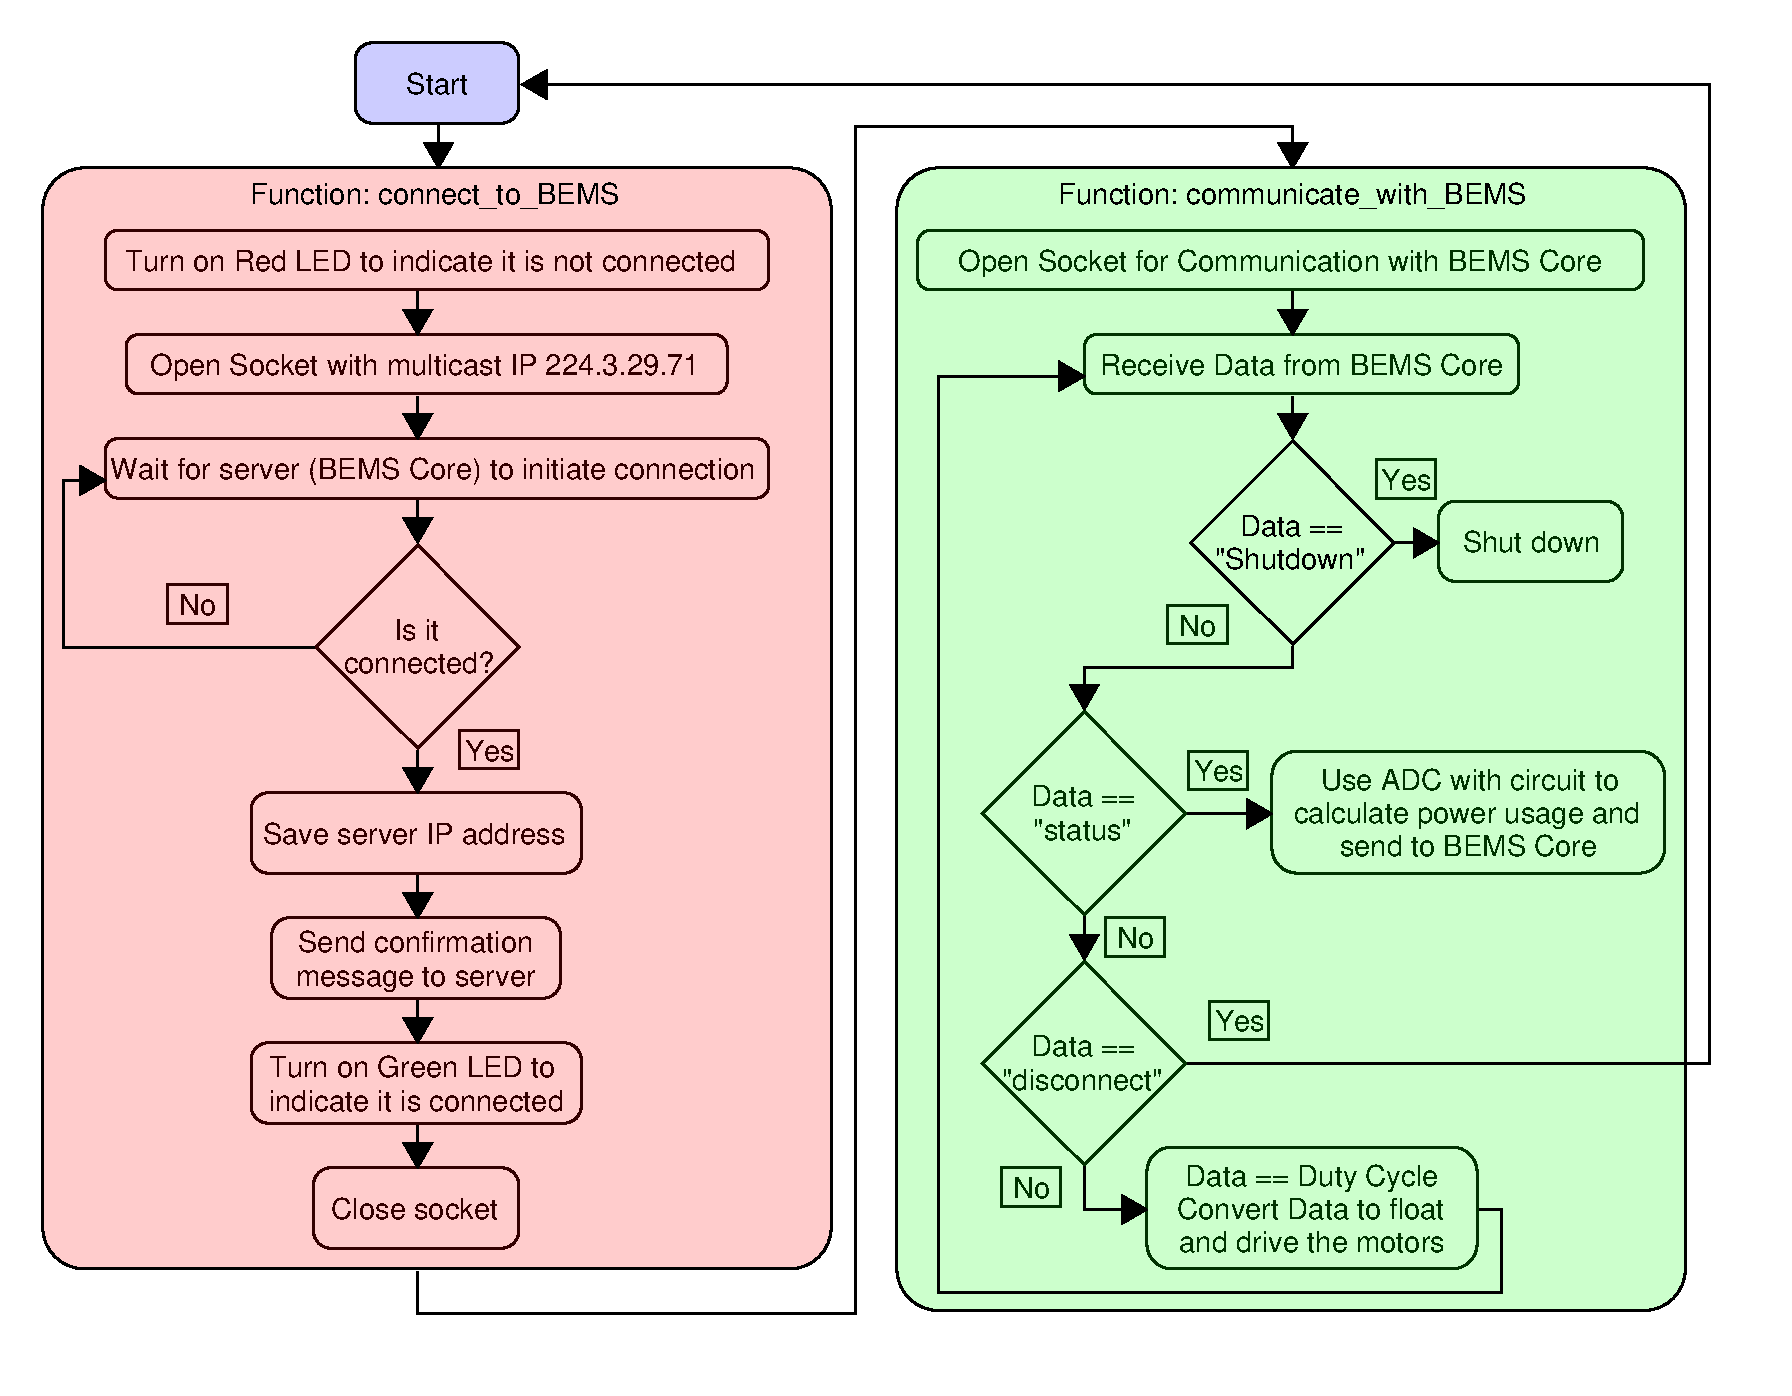
\includegraphics[scale=0.5]{figs/Beaglebone_Receiver_Diagram.pdf}
    \caption{Receiver Running on Embedded Computer}
    \label{fig:Beaglebone_Receiver_Diagram}
\end{figure}

The embedded computer needed some software to be able to connect to and communicate with the iBEMS Core. To achieve this, a program consisting of 2 functions for connecting and communicating is used.
\medbreak
The first of these functions is \texttt{connect\_to\_iBEMS}. This function first turns on the red LED on the embedded computer to indicate it is not yet connected. Then it creates a socket using a multicast IP address that the corresponding API in the iBEMS core will be looking for. Once the socket is created, the embedded computer will enter a loop and wait for the iBEMS core to make the initial connection. When that connection is made, it will exit the loop, save the IP address of the iBEMS core, send a confirmation message, then turn on the green LED before closing the multicast socket.
\medbreak
The second function, \texttt{communicate\_with\_iBEMS} will open another socket but with the IP address of the iBEMS core found in \texttt{connect\_to\_iBEMS}. It will then enter an indefinite loop to continually receive data from the iBEMS core. There are 4 different messages that the iBEMS core sends to the embedded computer. First, it will check if the iBEMS core is telling it to shut down with the command \say{Shutdown}. If so, the embedded computer will immediately shut down. Second, if the data sent by iBEMS is \say{status}, the embedded computer will take a reading from the circuit described in Chapter~\ref{ch: Chapter2} section 3. In case the user decides to shut down the iBEMS core without turning off the embedded computer, another message \say{disconnect} will be sent in which case the embedded computer will exit \texttt{communicate\_with\_iBEMS} and start the entire program over again. Finally, if iBEMS is not sending any of the above options, it means that the user is sending a new duty cycle to drive the motors with. Since iBEMS only sends messages with the string data type, this has to be converted to a float in order to call the motor driver function. 


%%% Local Variables:
%%% mode: latex
%%% TeX-master: "../finalReport"
%%% End:

\chapter{Experimental Results}
\label{ch: Chapter4}

As part of this project, we developed a working prototype. As explained in Chapter~\ref{ch: Chapter2} section 2, the first mode is the startup menu:

\begin{figure}[H]
    \centering
    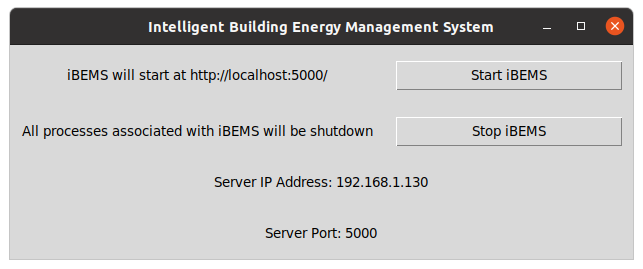
\includegraphics[scale=0.5]{figs/BEMS_GUI_Linux.png}
    \caption{Desktop GUI}
    \label{fig:desktopgui}
\end{figure}

\noindent
Here, the user will simply click the "Start iBEMS" button to launch the web
server and agents. When the user is finished, all agents and the web server can
be shut down by clicking "Stop iBEMS." In case the user accidentally clicks the
"Start iBEMS" button while iBEMS is already running, then the following error
message will appear:

\todo[inline]{Fix all the quotations}

\begin{figure}[H]
    \centering
    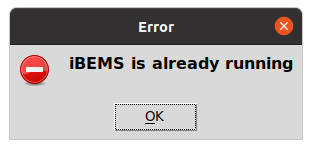
\includegraphics[scale=0.5]{figs/BEMS_GUI_Linux_Warning.png}
    \caption{Popup Error}
    \label{fig:popuperror}
\end{figure}

\noindent
After launching iBEMS, the web browser will open and the user will presented with the login page:

\begin{figure}[H]
    \centering
    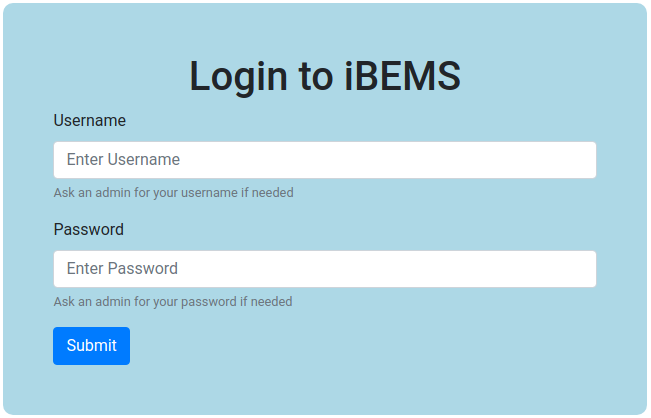
\includegraphics[scale=0.5]{figs/Login.png}
    \caption{Login Page}
    \label{fig:Home_screen}
\end{figure}

\noindent
where the user can enter in their username and password. Currently, iBEMS does not have a robust user login. It actually just has 1 username and password that is defined in the code. When the user enters the valid username and password, the home page will load automatically, where the weather data can be seen:

\begin{figure}[H]
    \centering
    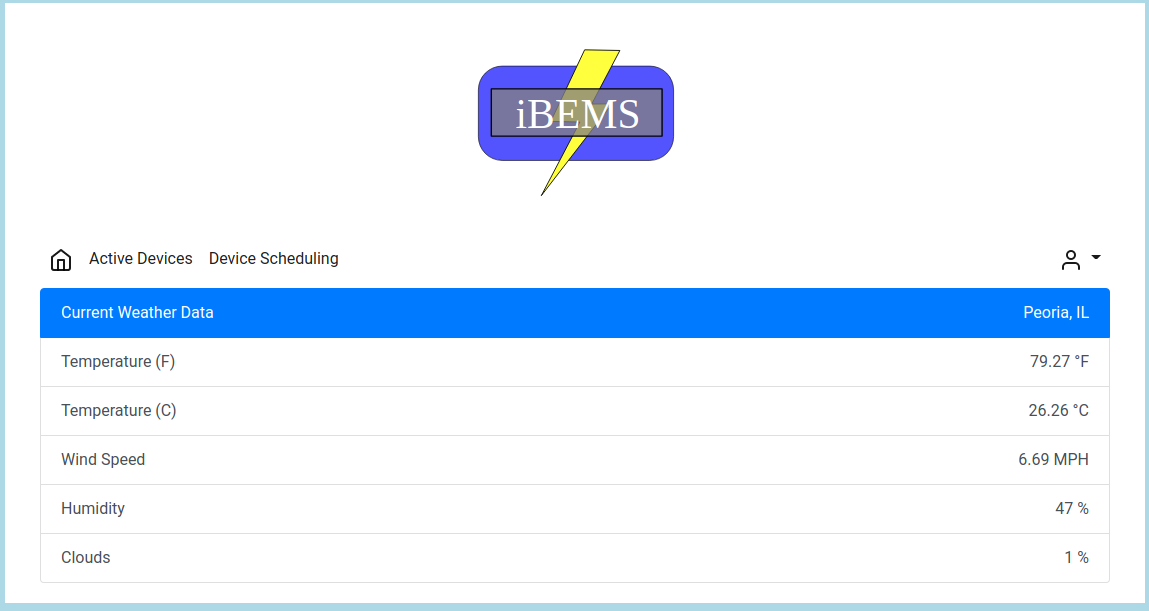
\includegraphics[scale=0.35]{figs/Home_screen.png}
    \caption{Home Page}
    \label{fig:Home_screen}
\end{figure}

The home screen (mode 2) does not have any interactive functionality other than to load another page by selecting one on the navigation bar.

\begin{figure}[H]
    \centering
    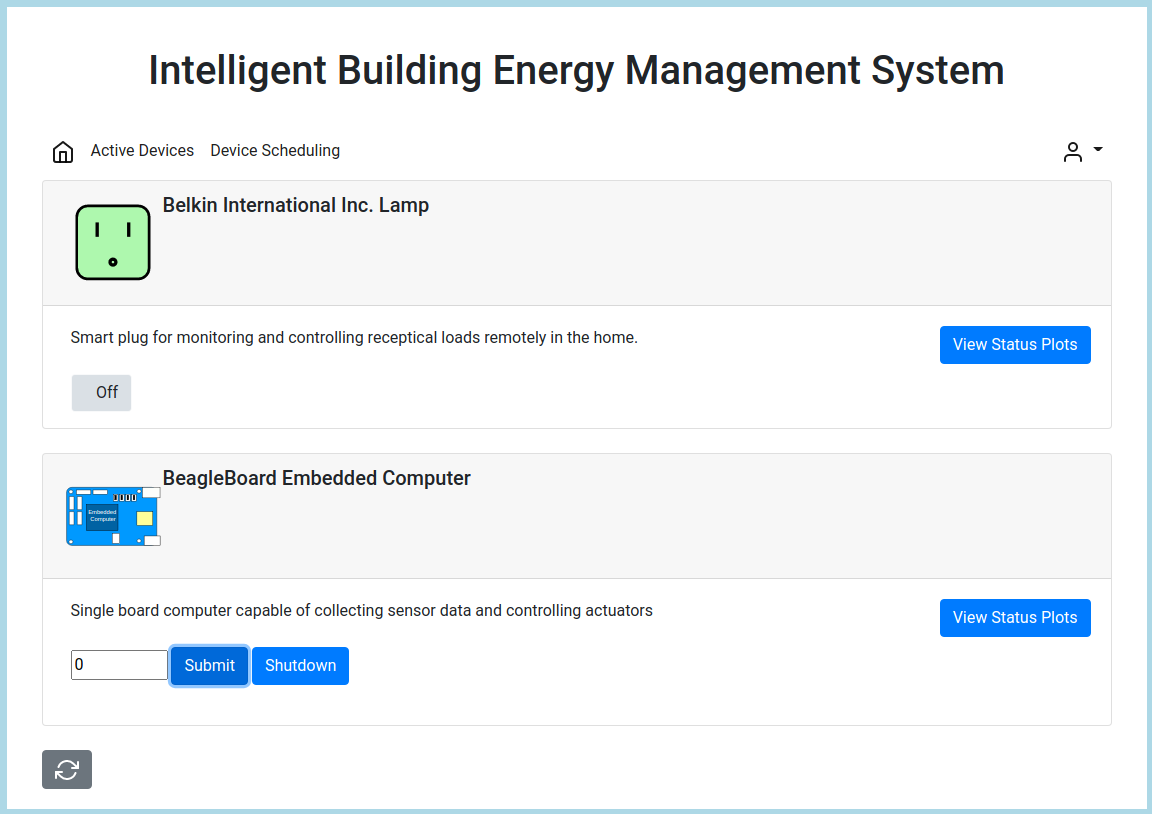
\includegraphics[scale=0.35]{figs/ActiveDevices_screen.png}
    \caption{Active Devices Page}
    \label{fig:active_devices}
\end{figure}

Figure~\ref{fig:active_devices} shows the active devices page (mode 3) which is loaded upon clicking "Active Devices" in the navigation bar. Here, all the connected devices are shown in order of when they connected to iBEMS. As mentioned previously, control of the WeMo Insight Switch is limited to turning it on and off while the embedded computer's motor speed can be controlled by submitting different duty cycles. Additionally, the embedded computer can be completely turned off by clicking the "Shutdown" button. Both supported devices also log their power usage at regular intervals. A plot of these power usage data points can be viewed by clicking "View Status Plots."

\begin{figure}[H]
    \centering
    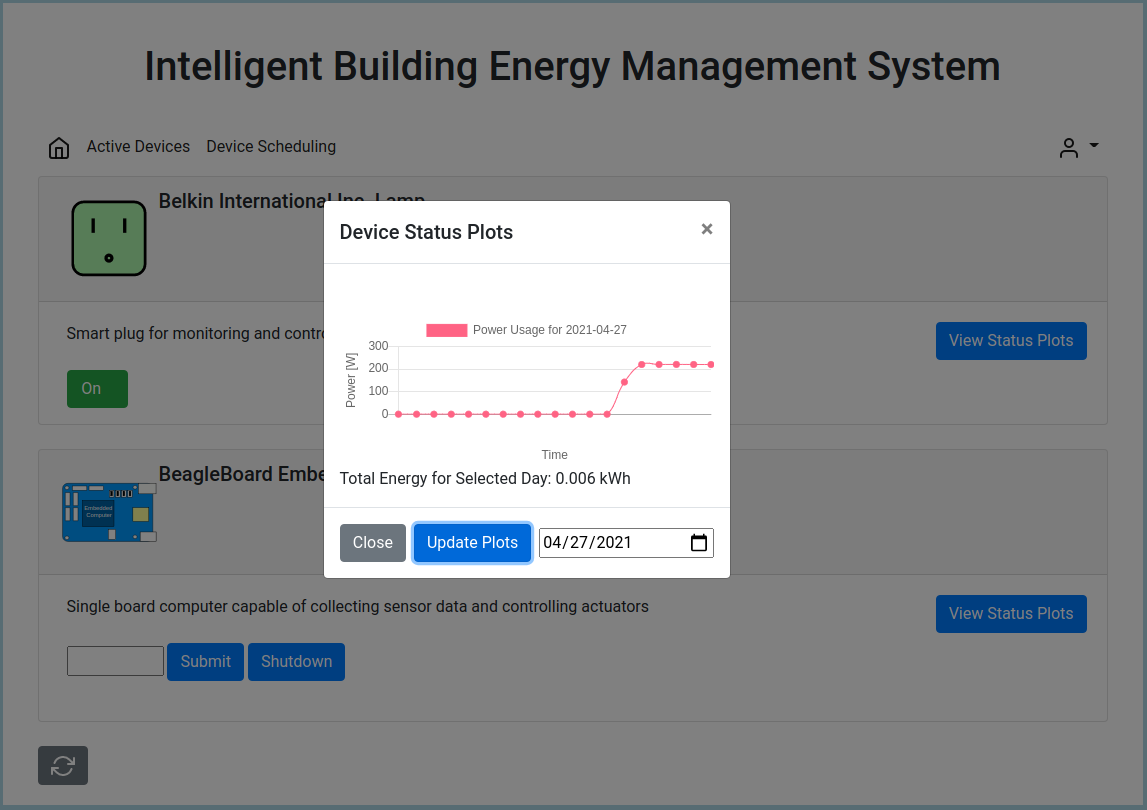
\includegraphics[scale=0.35]{figs/ActiveDevices_plot.png}
    \caption{Active Devices Plot}
    \label{fig:active_devices_plot}
\end{figure}

After clicking "View Status Plots," a modal will pop up for the user to further
interact with. By default, power usage data points for the current day are
loaded at first, but another day can be selected by clicking on the calendar
icon in the lower right corner. The plot is then updated by clicking "Update
Plots." This is done by collecting data from the Apache Cassandra database and
simply plotting all the points found for the specified day. Underneath the plot,
the total energy consumed for the specified day is displayed. That total energy
is found using the trapezoid method for integration on the plot. %
%
\begin{figure}
    \centering
    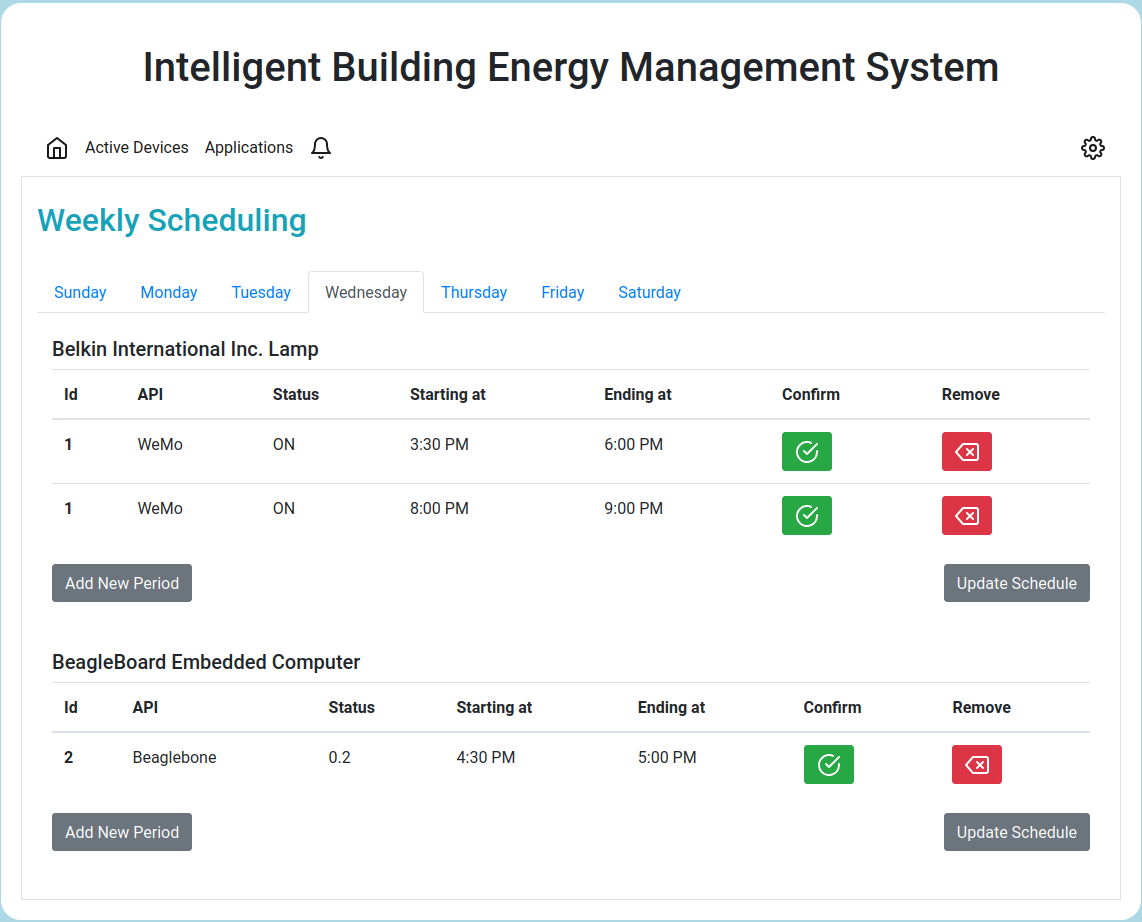
\includegraphics[scale=0.35]{figs/Applications_screen.png}
    \caption{Scheduling Page}
    \label{fig:schedulingl}
\end{figure}
%

Mode 4, or the scheduling page, can be loaded by clicking the "Device
Scheduling" button in the navigation bar. Much like the active devices page,
each connected device is listed in order of when they connected to iBEMS.
Instead of directly controlling the devices, the user can enter in time periods
when they want each device to maintain a specified status. For example, the WeMo
Insight Switch can be scheduled to be on from 5 to 8 P.M. on Fridays. Likewise,
the embedded computer can be scheduled to maintain a duty cycle of 0.5 for the
same time period every Friday. Scheduled times can be added with the "Add new
Period" and deleted by clicking the red "X" by the corresponding time period.

%%% Local Variables:
%%% mode: latex
%%% TeX-master: "../finalReport"
%%% End:

\chapter{Conclusion}
\label{ch: Chapter5}


\section{Advantages}
iBEMS is open source, easy-to-use, and was developed using a modular, agent-based code base. Being open source makes it freely available to anyone who has the supported devices and wants to begin managing their home energy usage. The simple interface is easy to figure out for less tech-savvy users and the modular code base makes this system relatively easy for others to continue development. 

\section{Disadvantages}
Despite its advantages, potential users should be aware of the rather obvious disadvantages at this point. A typical commercial building energy management system will include many more features like predicting future energy use and supporting more devices.

\section{Challenges}
The biggest challenges we foresee for future developers are adapting iBEMS to an enterprise network and adding the security necessary to do so. As mentioned before, iBEMS currently only works when all devices are connected through a single router. Scaling iBEMS up to an enterprise network with multiple access points will be an immensely complicated upgrade. Further more, security will be needed to make sure only select clients on an enterprise network will be able to login to iBEMS and have control over the connected devices. This will involve a much more robust login feature and possibly encrypting the messages being sent to and from the devices and iBEMS core.

\section{Future Work}
One of the main ways to improve the software is to refactor the user interface as the current interface is fairly primitive. Adding elements like collapsible drop down menus and a collapsible side bar would make the interface more professional and user-friendly. BEMOSS could be used as a reference in this process. Secondly, a better and more robust user login system could help decrease the risk of security breaches. Granular access control to different parts of the site could help ensure that only certain groups of individuals have access to certain features. An efficient way to implement this would be to use the add-on to Flask known as flask-login. To improve the overall reliability and speed of the software, a better agent communication protocol could be researched and implemented. Many problems are visible with the use of ZeroMQ as exceptions are thrown occasionally when device status updates are sent in quick succession to the control agent. Potentially, there exists a better solution than publish-subscribe. One of the major issues with the software is lack of device data persistence across system restarts. Developers in the future could help alleviate this problem by refactoring the device storage system in the Cassandra database.

% \input{parts/20-modeling2-DOF.tex}
% \input{parts/30-controlAlgorithms.tex}
% \input{parts/40-simulations.tex}
% \input{parts/50-implementation.tex}
% \input{parts/60-conclusion.tex}

% %----------------------------------------------------------------------
% % APPENDICES
% %---------------------------------------------------------------------- 
\appendix
% % Designate with \appendix declaration which just changes numbering style 
% % from here on
% % Add a title page before the appendices and a line in the Table of Contents
\addcontentsline{toc}{chapter}{APPENDICES} 
% %

\chapter{Installation}
\label{ap: appendixA}

This appendix provides the steps for installing iBEMS on Ubuntu or any supported distribution of Linux.

\section{Cloning the repository}
The first step is to clone the repository with the command.
\begin{verbatim}
    git clone -b master https://github.com/ejwatkins
    /seniorProject1-2020-21-Code.git
\end{verbatim}
This will clone the master branch of the private Github repository owned by Elliot Watkins. It is recommended to run this command in the Unix user's home directory to find it easily.
\begin{figure}[H]
    \centering
    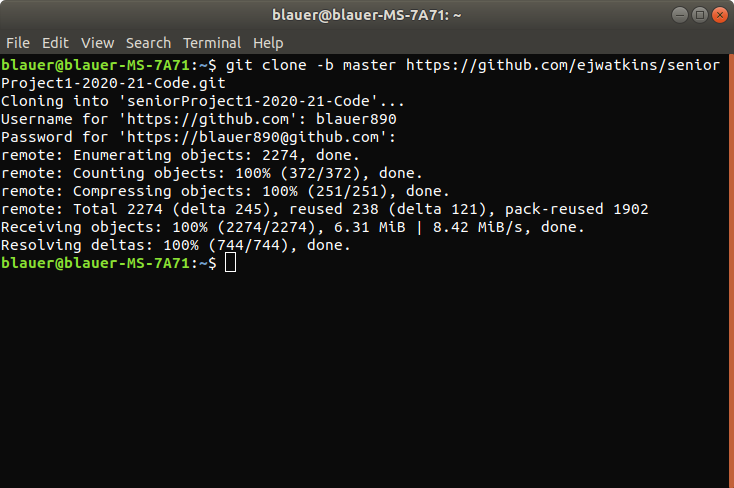
\includegraphics[scale=0.4]{figs/cloneiBEMS.png}
    \caption{Cloning iBEMS}
    \label{fig:cloneibems}
\end{figure}
If no errors occurred, terminal output similar to Figure~\ref{fig:cloneibems} will appear. A directory titled \texttt{seniorProject-2020-21-Code} will appear in the user's home directory.

\section{Creating the virtual environment}
Before the system can be properly installed, a Python 3 virtual environment must be created. After changing into the source code directory, this can be performed with the command
\begin{verbatim}
    python3 -m venv venv
\end{verbatim}
The final argument supplies the name of the directory the virtual environment will be placed in. For now, the name of the directory must be \texttt{venv} as this path name is hard coded in the source code. No terminal output should be generated when running this command if the proper version of Python 3 is installed along with the virtual environment package. If no errors occur, output similar to that of Figure~\ref{fig:createvenv} will be shown.

\begin{figure}[H]
    \centering
    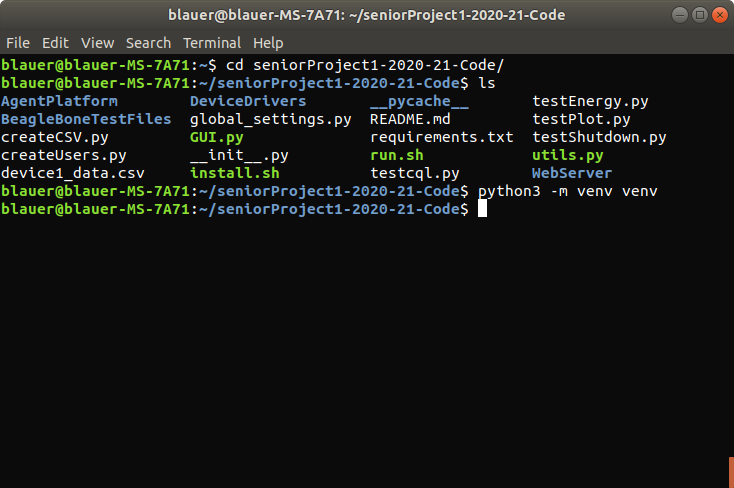
\includegraphics[scale=0.4]{figs/createvenv.png}
    \caption{Creating the virtual environment}
    \label{fig:createvenv}
\end{figure}

\section{Running the installation script}
Once the venv is created, the platform will be able to be properly installed by running the command
\begin{verbatim}
    ./install.sh
\end{verbatim}
If this script does not have executable permission for the current user, the following command will change the permissions of the file to allow it to be run by any normal user:
\begin{verbatim}
    chmod u+x install.sh
\end{verbatim}
This script will run through and install any necessary Python packages via the \texttt{requirements.txt} file, install the Apache Cassandra database, and place necessary project directories on the PYTHONPATH. Output similar to that in Figure~\ref{fig:runinstall} will be produced.

\begin{figure}[H]
    \centering
    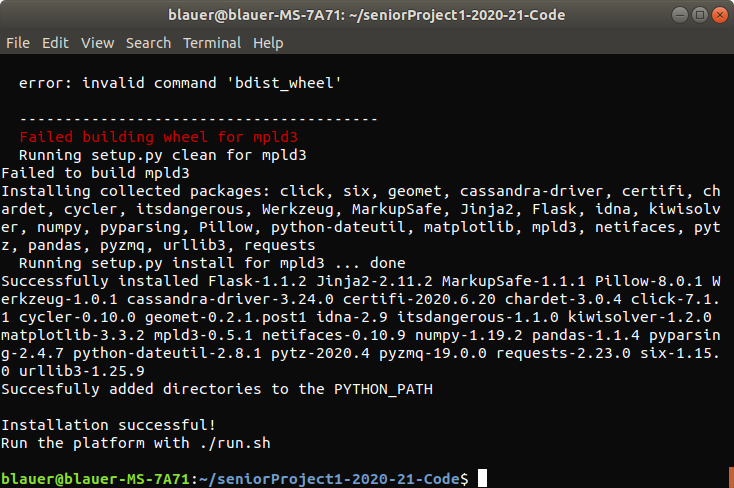
\includegraphics[scale=0.4]{figs/runinstall.png}
    \caption{Running the installation script}
    \label{fig:runinstall}
\end{figure}
An error regarding the installation of the \texttt{mpld3} package may be visible. However, this can be ignored as this package is not used in the current version of the software.
\medbreak\noindent
At this point, the software can be started with the \texttt{GUI.py} Python script.
\chapter{How to Run}
\label{ap: appendixB}

This appendix describes the few steps that are required to get the software running on the user's Linux machine.

\section{Running the Python GUI}
In the top level directory of the project, there should be a file titled \texttt{GUI.py} which will act as the main entry point into the project. To run this file, it can be run either as an executable with
\begin{verbatim}
    ./GUI.py
\end{verbatim}
or as a Python script with
\begin{verbatim}
    python3 GUI.py
\end{verbatim}
The output GUI is shown in Figure~\ref{fig:desktopGUI}
\begin{figure}[H]
    \centering
    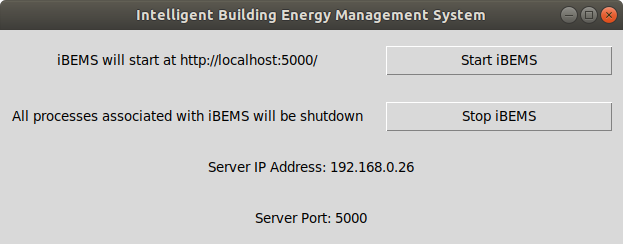
\includegraphics[scale=0.5]{figs/desktopGUI.png}
    \caption{Desktop GUI}
    \label{fig:desktopGUI}
\end{figure}

\section{Running the software}
By clicking on the "Start iBEMS" button shown in Figure~\ref{fig:desktopGUI}, the software will be launched in a new terminal shown in Figure~\ref{fig:runningterminal}.
\begin{figure}[H]
    \centering
    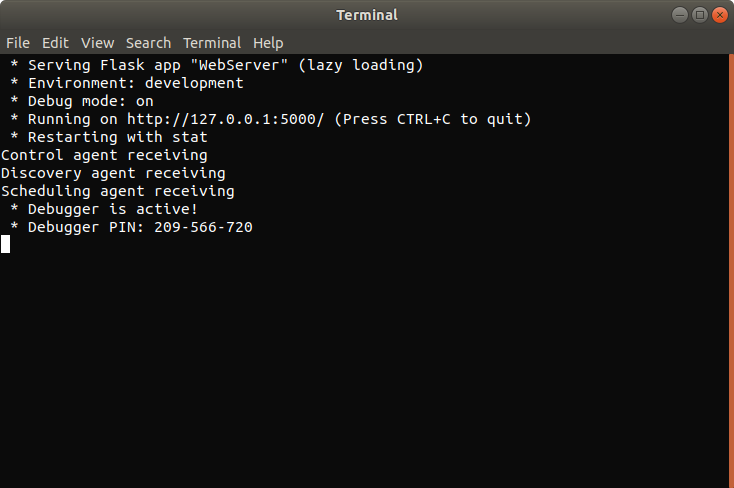
\includegraphics[scale=0.4]{figs/runningterminal.png}
    \caption{Running terminal}
    \label{fig:runningterminal}
\end{figure}

\chapter{WeMo Insight Switch Setup}
\label{ap: appendixC}

This appendix describes the steps required to connect the WeMo Switch to a WiFi network. A prerequisite requires downloading the Wemo app from Google Play or the Apple App Store. In order to initiate the connection process, the WeMo must be plugged into an outlet while holding down the the reset button for 5 seconds. This should allow the WeMo to broadcast its own WiFi network titled \say{WeMo.Insight.23A}. This WiFi network must be connected to allow the device to be paired with the desired network.

\section{Create a WeMo account}
If the app was recently downloaded, a screen shown in Figure~\ref{fig:signInWemo} is displayed where the user can either create an account or sign in with an existing account.
\begin{figure}[H]
\centering
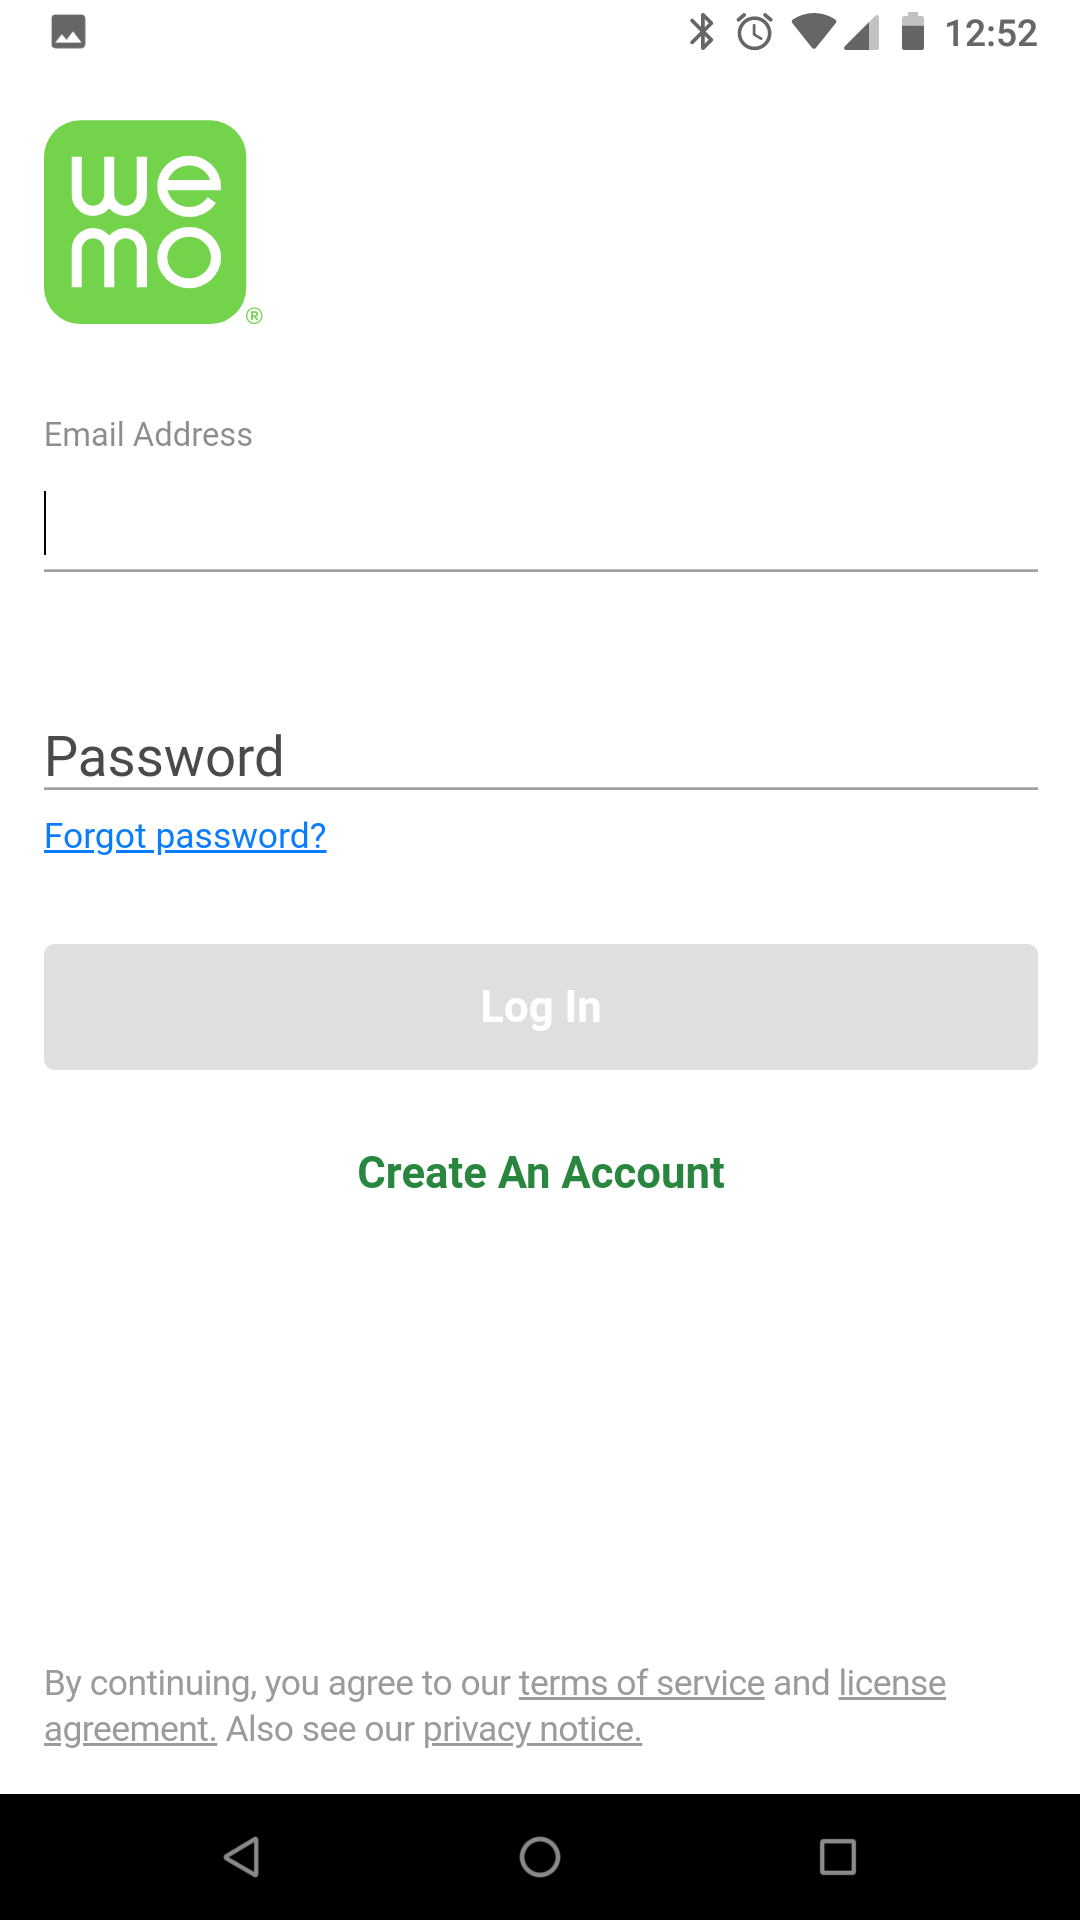
\includegraphics[scale=0.09]{figs/wemoApp/signInWemo.png}
\caption{WeMo app sign-in page}
\label{fig:signInWemo}
\end{figure}

\section{Name the device}
A screen will appear asking the user to enter the friendly name of the device as in Figure~\ref{fig:nameDevice}
\begin{figure}[H]
\centering
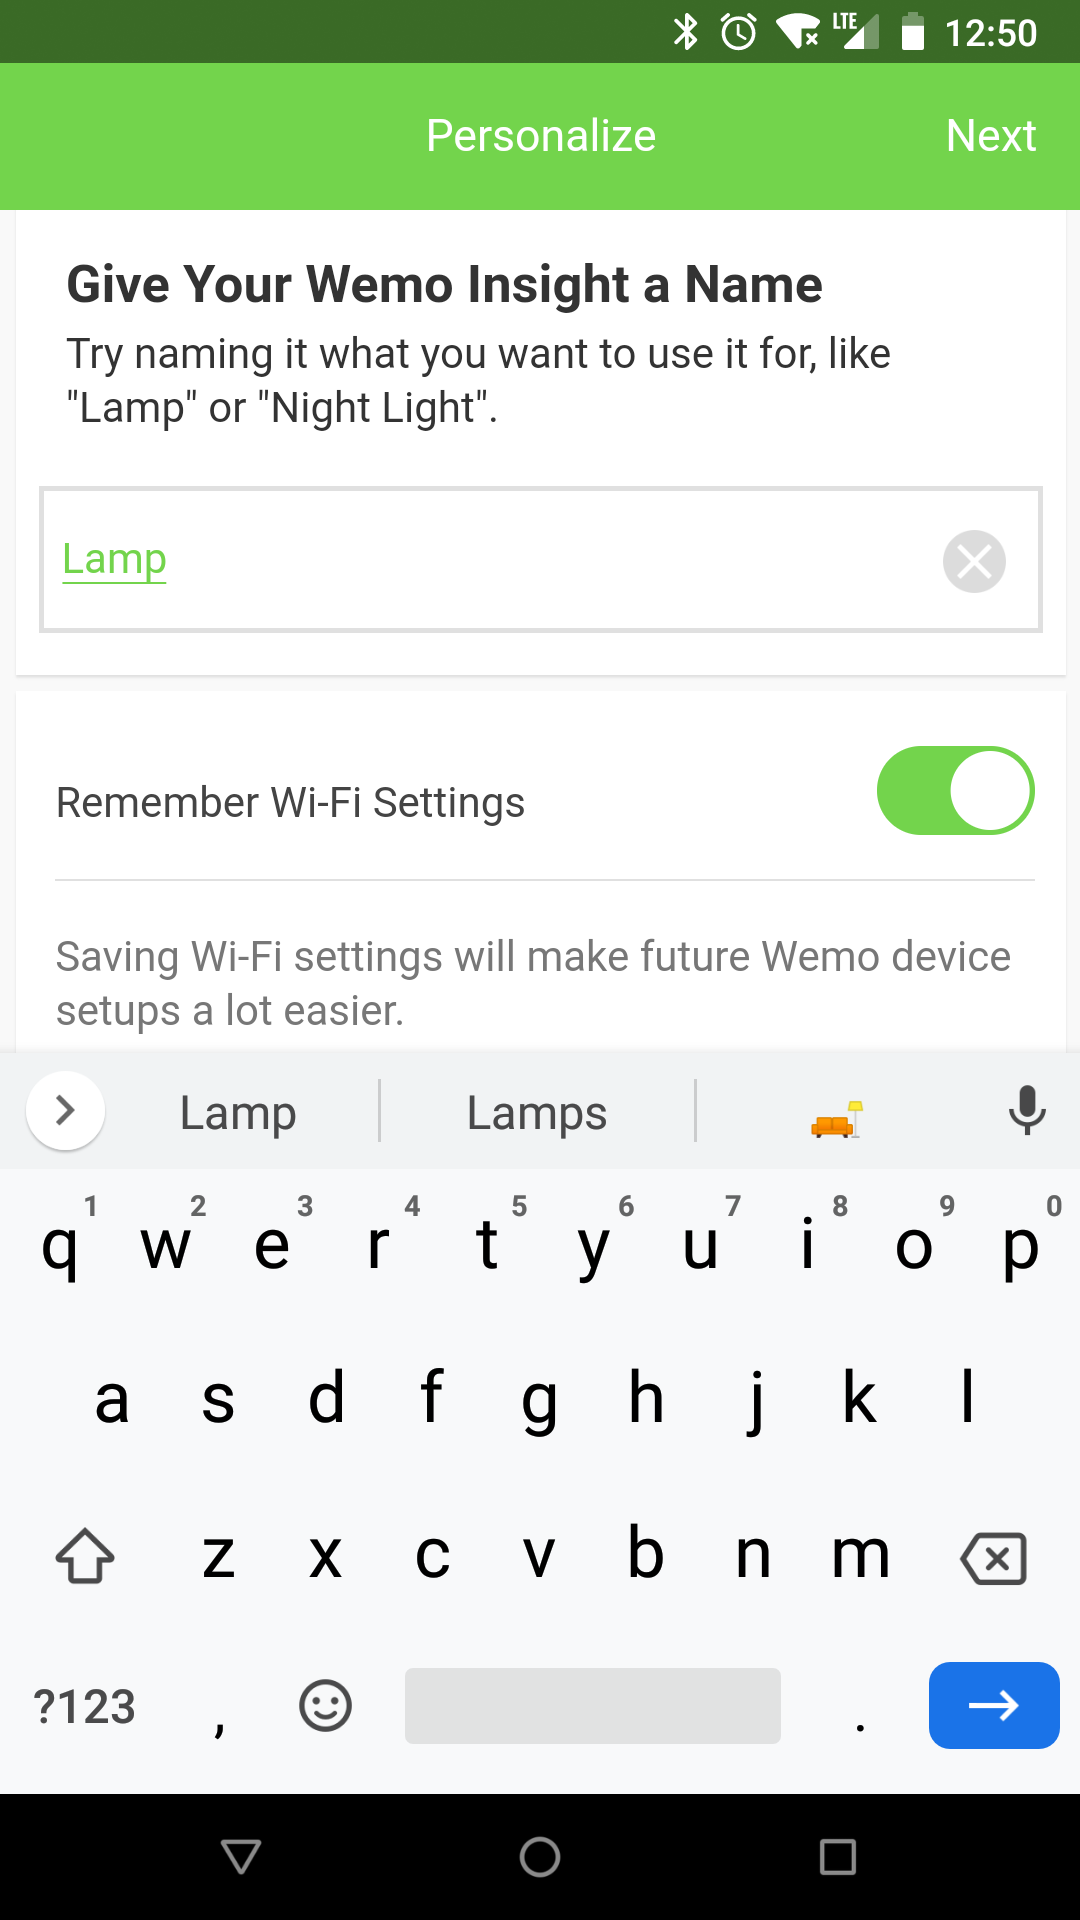
\includegraphics[scale=0.09]{figs/wemoApp/nameDevice.png}
\caption{Name device page}
\label{fig:nameDevice}
\end{figure}

\section{Pair WiFi network with the WeMo}
If the plug's WiFi network is connected to on the user's phone, the user will be prompted to connect to the desired WiFi network. Once this pairing is complete the screen in Figure~\ref{fig:completedSetup} will appear.
\begin{figure}[H]
\centering
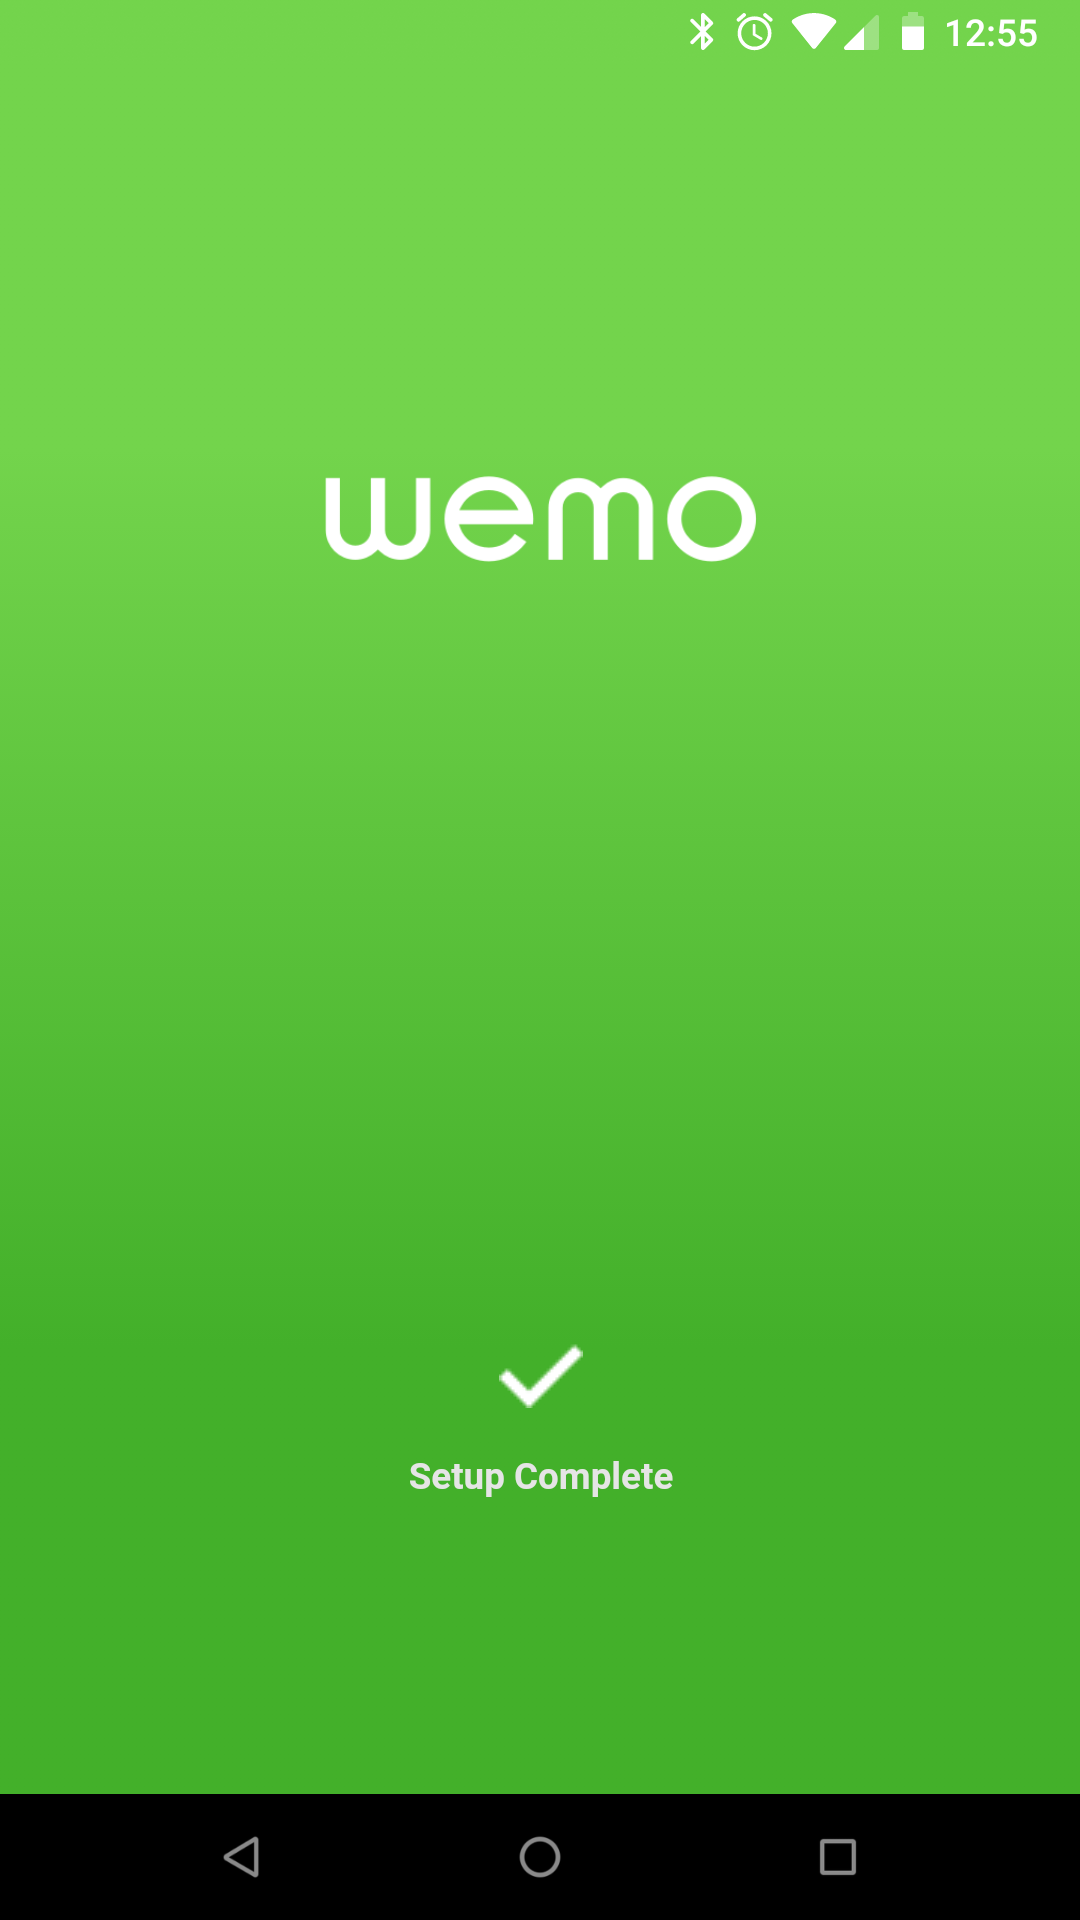
\includegraphics[scale=0.09]{figs/wemoApp/setupComplete.png}
\caption{Completed setup}
\label{fig:completedSetup}
\end{figure}

\section{Control the WeMo}
If everything was setup successfully, the user should be able to turn on and off the WeMo and see the power usage as in Figure~\ref{fig:smartPlutControl}.
\begin{figure}[H]
\centering
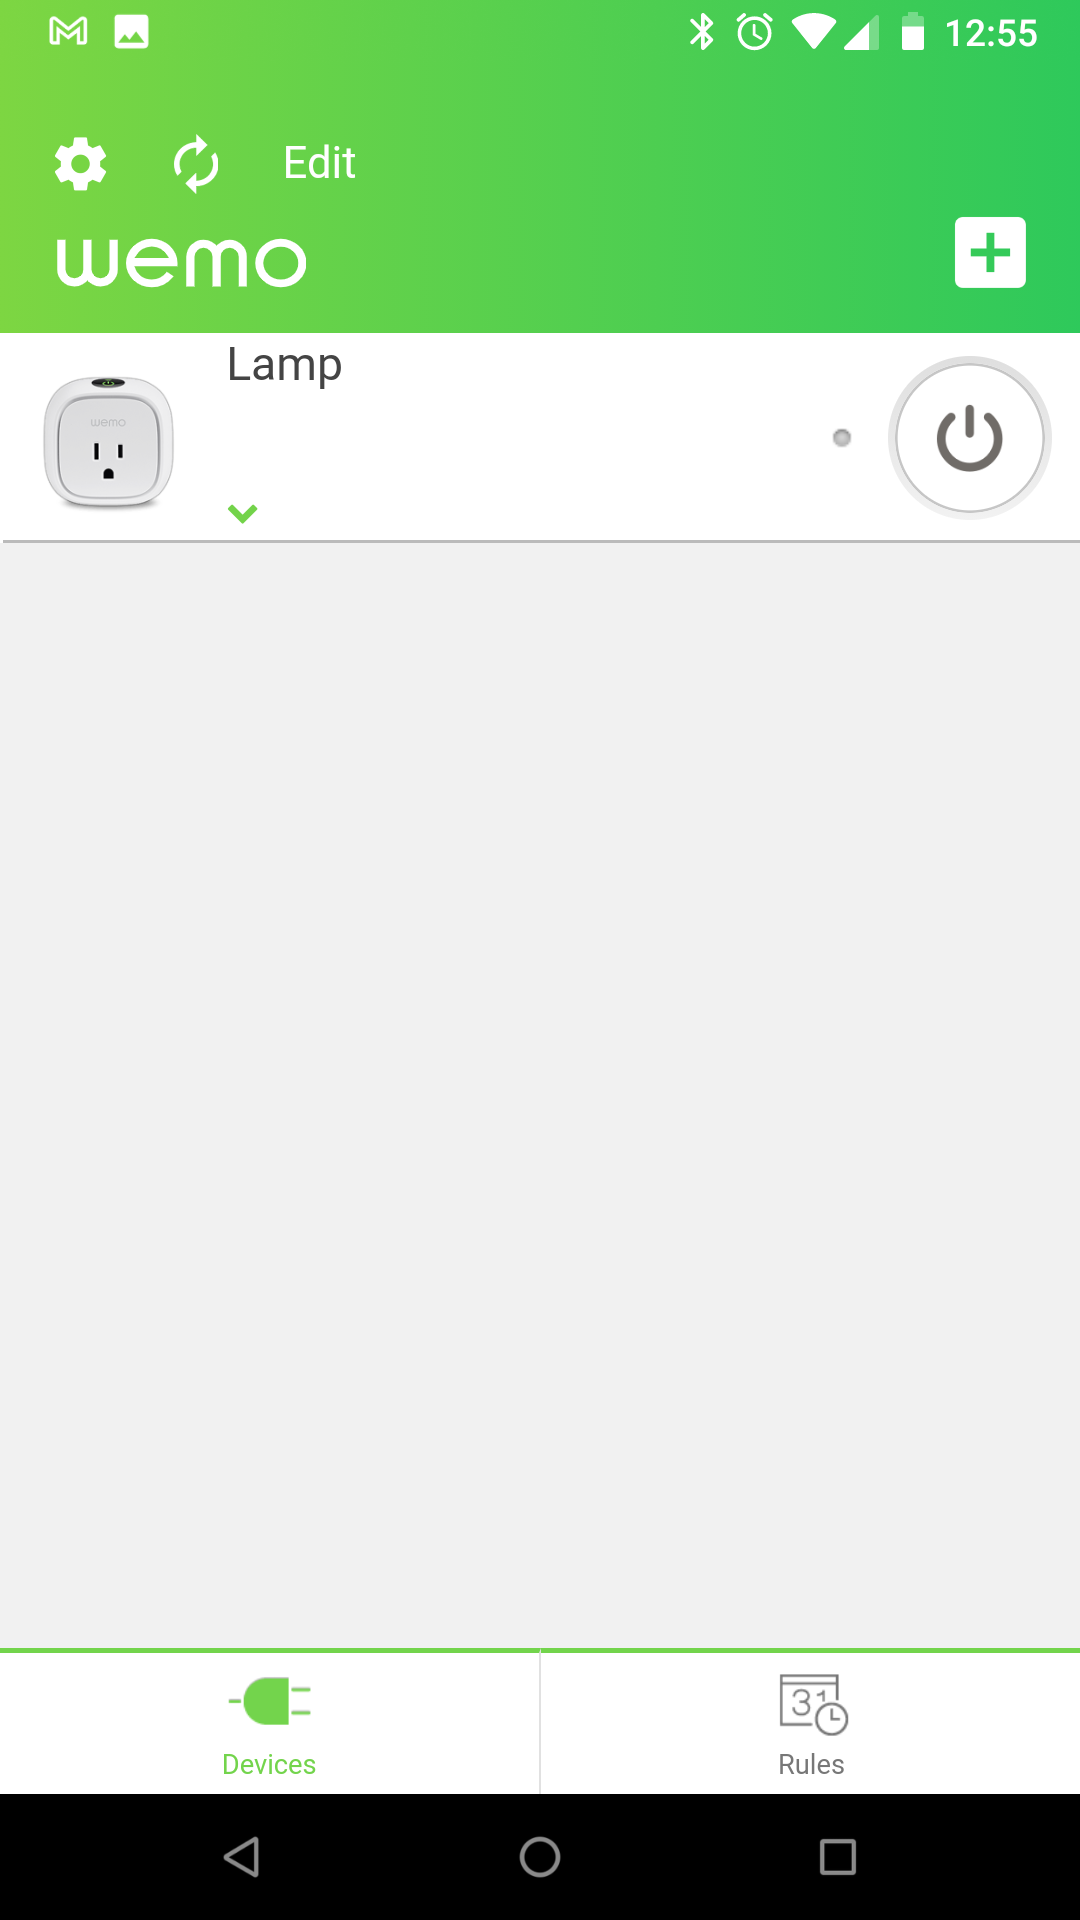
\includegraphics[scale=0.09]{figs/wemoApp/wemoAppControl.png}
\caption{Control the smart plug}
\label{fig:smartPlutControl}
\end{figure}

If any problems were encountered during the setup process, the user can go to\\
\href{https://www.wemo.com/support/}{https://www.wemo.com/support/}. Also, the paper manual provided with the WeMo box can provide additional support as it provides a comprehensive step-by-step process.
\chapter{Embedded Computer Setup}
\label{ap: appendixD}

This appendix describes the steps required to connect an embedded computer to the iBEMS Core. 

\section{Connect to router}
In our project, we used a BeagleBone Blue for the embedded computer. To connect to your specific router, first plug in the BeagleBone Blue to your computer with a microUSB cable. Then open a terminal and install \say{screen} with the command \say{sudo apt install screen}. You will then need to find the USB driver being used for the beaglebone with \say{dmesg}. Scroll through the information until you find the BeagleBone:

\begin{figure}[H]
\centering
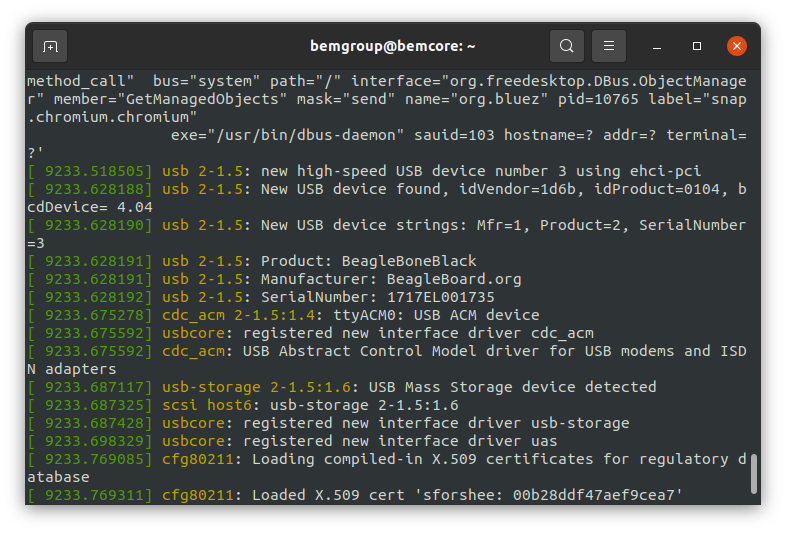
\includegraphics[scale=0.4]{figs/beaglebone/findUSBdriver.png}
\caption{Finding USB Driver}
\label{fig:bb_findUSB}
\end{figure}

In Figure~\ref{fig:bb_findUSB}, it can be seen that \say{ttyACM0} is the USB driver being used.

With that knowledge, you can now enter the command \say{sudo screen /dev/ttyACM0} to login into the Beaglebone Blue. Enter username \say{debian} and password \say{temppwd} to login.
\medbreak
Once you are logged into the Beaglebone Blue, follow these instructions to connect to your router:
\href{http://www.strawsondesign.com/\#!manual-wifi}{http://www.strawsondesign.com/\#!manual-wifi}.

\section{Copy Necessary Files}
Now that the Beaglebone Blue is connected to the router, you need to copy some files to it. First, find the IP address of the BeagleBone Blue with the command \say{ifconfig wlan0}:

\begin{figure}[H]
\centering
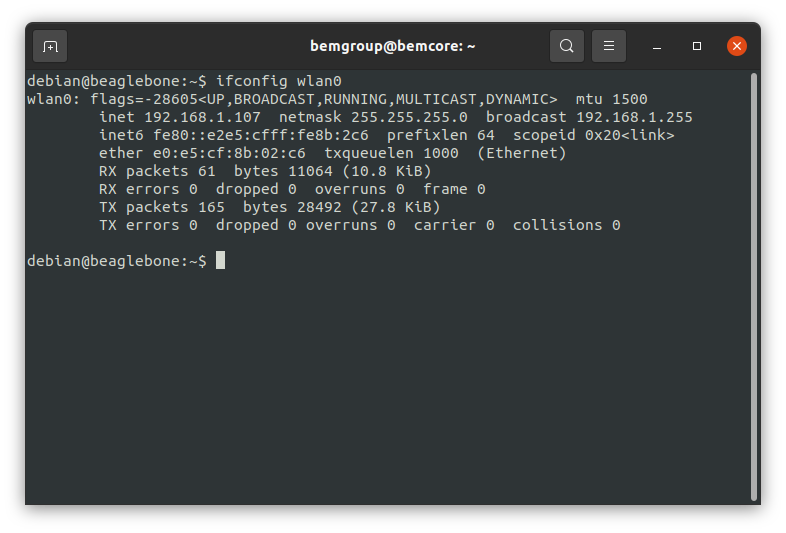
\includegraphics[scale=0.4]{figs/beaglebone/findIPaddress.png}
\caption{Finding IP Address}
\label{fig:bb_findIP}
\end{figure}

Figure~\ref{fig:bb_findIP} shows the output of \say{ifconfig wlan0} and it can be seen that the IP address in this case is \texttt{192.168.1.107}.
\medbreak
You can now open a new native linux terminal and go the the \say{seniorProject1-2020-21-Code} directory. Once there, copy the necessary files with commands:
\\
\say{scp BeagleboneReceiver.py debian@192.168.1.107:/home/debian},
\\
\say{scp BeagleBoneSupportFiles/LED.py debian@192.168.1.107:/home/debian},
\\
\say{scp BeagleBoneSupportFiles/PWM.py debian@192.168.1.107:/home/debian}.
You may get a warning message about the authenticity of the host, but simply type \say{yes} as response to this warning.

\section{Running the BeagleBone Receiver}
With the necessary files on the BeagleBone Blue, you can go back the BeagleBone Blue terminal and enter the command \say{python3 BeagleboneReceiver.py}. Finally, you can start iBEMS and it will connect to the Beaglebone Blue automatically.
% \input{parts/B-simulation.tex}
% %\input{parts/C-USB.tex}
% \input{parts/D-RP.tex}
% \input{parts/E-ADP.tex}
% \input{parts/tutorial.tex}

% %----------------------------------------------------------------------
% % END MATERIAL
% %----------------------------------------------------------------------

% % B I B L I O G R A P H Y
% % -----------------------
% %
% % The following statement selects the style to use for references.  It controls the sort order of the entries in the bibliography and also the formatting for the in-text labels.
\bibliographystyle{plain}
% % This specifies the location of the file containing the bibliographic information.  
% % It assumes you're using BibTeX (if not, why not?).
% \ifthenelse{\boolean{PrintVersion}}{
% \cleardoublepage % This is needed if the book class is used, to place the anchor in the correct page,
%                  % because the bibliography will start on its own page.
% }{
% \clearpage       % Use \clearpage instead if the document class uses the "oneside" argument
% }
% \phantomsection  % With hyperref package, enables hyperlinking from the table of contents to bibliography             
% % The following statement causes the title "References" to be used for the bibliography section:
% % \renewcommand*{\bibname}{References}
% Bibliography 
\renewcommand{\bibname}{Bibliography}

% Add the References to the Table of Contents
\addcontentsline{toc}{chapter}{\textbf{References}}

\bibliography{bib/references}
% Tip 5: You can create multiple .bib files to organize your references. 
% Just list them all in the \bibliogaphy command, separated by commas (no spaces).

%
% @online{BEMOSS,
%   author = {Virginia Tech},
%   title = {BEMOSS3.5},
%   year = 2019,
%   url = {https://github.com/bemoss/BEMOSS3.5},
%   urldate = {2010-09-30}
% }

% @online{zeromq,
%   author={zeromq},
%   title={ZeroMQ},
%   year = {2021},
%   url = {https://zeromq.org/},
% }

%----------------------------------------------------------------------
\end{document}
%======================================================================



%%% Local Variables: 
%%% mode: latex
%%% TeX-master: t
%%% End: 